\documentclass[a4paper,10pt]{scrartcl}
\usepackage[utf8]{inputenc}
\usepackage[T1]{fontenc}
\usepackage{booktabs}
\usepackage{import}
\usepackage{xspace}
\usepackage{enumitem}
\usepackage{cite}
\usepackage{graphicx}
\usepackage{tikz}
\usepackage{wrapfig}
\usepackage{tikz-uml}
\usepackage{gantt}
\usepackage{pdflscape}
\usetikzlibrary{arrows}
\usetikzlibrary{fit}
\usetikzlibrary{calc}
\usepackage{float}
\usepackage{amssymb}
\usepackage{listings}
\usepackage[section]{placeins} % don't move figures beyond the next section heading

% this is needed for forms and links within the text
\usepackage{hyperref}

% Variables
\newcommand{\authorName}{
   Mohammed~Abu~Jayyab,
   Niklas~Baumstark,
   Tobias~Gräf,
   Amrei~Loose,
   Christoph~Michel,
}
\newcommand{\authorNameEmph}{
   Mohammed~Abu~Jayyab,
   Niklas~Baumstark,
   \textbf{Tobias~Gräf},
   Christoph~Michel,
   Amrei~Loose,
}

\newcommand{\dateFirstVersion}{\today}
\newcommand{\customer}{Karlsruhe Institute of Technology}
\newcommand{\contractor}{A company}
\newcommand{\projectName}{Broadcast Encryption\xspace}

\newcommand{\doctitle}{\projectName (Design document)}
\title{\doctitle}
\author{\authorName}
\date{\today}

% less margin
\usepackage[margin=2.5cm]{geometry}

% horizontal line
\newcommand{\HRule}{\rule{\linewidth}{0.5mm}}

% more beautiful lists
\setlist{noitemsep}
\renewcommand{\labelitemi}{$\bullet$}
\renewcommand{\labelitemii}{$\diamond$}

% create a shorter version for tables
\newcommand\addrow[2]{#1 &#2\\ }
\newcommand\addheading[2]{\textbf{\sffamily #1} &\textbf{\sffamily #2}\\ \hline}
\newcommand\tabularhead{\begin{tabular}{lp{13cm}}
\hline
}

\newcommand\addmulrow[2]{ \begin{minipage}[t][][t]{2.5cm}#1\end{minipage}%
   &\begin{minipage}[t][][t]{8cm}
    \begin{enumerate} #2   \end{enumerate}
    \end{minipage}\\ }

\newenvironment{usecase}{\tabularhead}
{\hline\end{tabular}}

% a cross
\newcommand\X{$\times$}

% templates and default styles for figures and graphics
\tikzset{>=triangle 45}
\tikzset{font=\sffamily}

\newcommand{\tmpCaption}{}
\newenvironment{illustration}[1]
{
   \renewcommand{\tmpCaption}{#1}
   \begin{figure}[ht!]
   \centering
}
{
   \caption{\tmpCaption}
   \end{figure}
}

% code
\lstset{frame=tRBl, frameround=tttt, basicstyle=\footnotesize\ttfamily}
\lstset{numbers=left, numberstyle=\scriptsize}
\lstset{tabsize=4}
\lstset{language=Java}


\begin{document}

\maketitle
  \begin{tabular}[t]{ll}
	Projekt:       & \quad \projektName \\[1.2ex]
	Auftraggeber:  & \quad \auftraggeber\\[1.2ex]
	Auftragnehmer: & \quad \auftragnehmer\\[1.2ex]
  \end{tabular}

\begin{tabular}{|p{3 cm}|p{3 cm}|p{5 cm}|}
\hline
\textbf{Version} & \textbf{Datum} & \textbf{Autor(en)} \\
\hline
\hline
1.0 & 29.04.2012 & \authorName \\
\hline
\end{tabular}
\clearpage

\tableofcontents
\clearpage

\section{Introduction}
%CryptoCast is a piece of software that provides a service to send contents from a central server to a given
%group of recipients. Transmission happens via a unidirectional communication channel like IP multicast.
%The traffic duplication that would be required for commonly used transport protocols is therefore avoided.

%It enables access control through a specific form of encryption that is based on the Naor-Pinkas broadcast
%encryption scheme. The advantage of this scheme is the 

The software CryptoCast will provide a service for sending encrypted data from a server to certain
amount of people.  This will be implemented as an unidirectional connection that makes it possible for the server
to send data without knowing how many people are receiving it and without the amount of traffic caused
by a bidirectional connection.  Also the type of the sent data will not be determined by the software. So it can be
used for all sorts of data exchange. For demonstration purposes we will implement a simple audio or video stream.

The server will be able to register new users and revoke specific persons if they are not allowed to receive the cast anymore. 
The client is an app on an Android smart phone that is used for receiving, decoding and displaying the data. 
The transport between them will be implemented with TCP but that can be replaced by another transport protocoll.

The implemented encryption algorithm will be the one by Moni Naor and Benny Pinkas, but later every other fitting the
interface can be used. This is important because there might be another more effective algorithm that can replace the implemented one.

In our design we will therefore focuse on modularity and encapsulation to enable substitution for parts of the programm without having to 
change a lot of their enviroment.

\section{Structure}
\subsection{Architecture}

We implement a server-client architecture with one central server sending the stream and multiple clients receiving it.

\begin{illustration}{packages}

\tikzset{
  rect/.style={draw,fill=green!15,minimum height=0.8cm,rectangle},
  box/.style={
    draw=blue!50!white,
    line width=1pt,
    dash pattern=on 1pt off 4pt on 6pt off 4pt,
    inner sep=4mm, rectangle, rounded corners
  },
}

\begin{tikzpicture}[auto,node distance=1.5cm]

\node[rect,minimum width=3cm](util) {cryptocast.util};
\node[rect,minimum width=3cm, below of=util](server) {cryptocast.server};
\node[rect,minimum width=3cm, xshift=3cm, right of=server](client) {cryptocast.client};
\node[rect,minimum width=3cm, xshift=3cm, right of=client](file) {cryptocast.client.filechooser};
\node[rect,minimum width=3cm, below of=server](crypto) {cryptocast.crypto};
\node[rect,minimum width=3cm, xshift=3cm, right of=crypto](naor) {cryptocast.crypto.naorpinkas};
\node[rect,minimum width=2cm, below of=crypto](comm) {cryptocast.comm};

\draw [<-] (util.south) -- ( server.north)
             node[pos=.5]{uses};

\draw [->] (server.south) -- (crypto.north)
             node[pos=.5]{uses};
\draw [->] (crypto.south) -- (comm.north)
             node[pos=.5]{uses};
\draw [->] (crypto.east) -- (naor.west)
             node[pos=.5]{uses};
\draw [->] (client.east) -- (file.west)
             node[pos=.5]{uses};

\end{tikzpicture}

\end{illustration}


The server will be designed with a three layer architecture, containing layers for presentation, application and data. In our case 
the presentation layer is presented by the shell, the application layer consists of the controller and the data layer contains ServerData and Command. Dividing the server into those layers makes the different parts less complex and it is possible to modify one layer without having to change the others.

\begin{illustration}{3-tier architecture of the server}

\tikzset{
  rect/.style={draw,fill=green!15,minimum height=0.8cm,rectangle},
  box/.style={
    draw=blue!50!white,
    line width=1pt,
    dash pattern=on 1pt off 4pt on 6pt off 4pt,
    inner sep=4mm, rectangle, rounded corners
  },
}

\begin{tikzpicture}[auto,node distance=1.5cm]

\node[rect,minimum width=6cm](shell) {\textbf{Shell}};
\node[rect,minimum width=3cm,xshift=-1.5cm,below of=shell](control) {Controller};;
\node[rect,minimum width=3cm,below of=control](data) {ServerData};
\node[rect,minimum width=2cm,xshift=2cm, right of=data](cmd) {Command};

\draw [<->]  (shell.south) --  (control.north)
;
\draw [->]  (shell.south) --  (cmd.north)
  ;
\draw [->]  (control.south) --  (data.north)
  ;

\end{tikzpicture}

\end{illustration}

\section{Package description}

\subsection{Package \lstinline!cryptocast.comm!}

\subsubsection{Class \lstinline|WritableByteChannelAdapter|}
Adapter to use a \lstinline|WritableByteChannel| (for example, a file or socket instance) as
 an \lstinline|OutChannel|. \\
\noindent\begin{minipage}[t]{5cm}
\vspace{0.3em}
\hspace*{2em}
\begin{tikzpicture}
\umlclass[]{WritableByteChannelAdapter}{

}{
+ send(data : byte[])
}
\end{tikzpicture}
\vspace{0.3em}
\end{minipage}



\textbf{\sffamily Superclasses and Interfaces}
\begin{itemize}
\item \lstinline|cryptocast.comm.OutChannel|
\end{itemize}


\textbf{\sffamily Constructors}
\begin{itemize}
\item \lstinline|public| \lstinline|WritableByteChannelAdapter|\lstinline|(WritableByteChannel inner)|\\ \\[-0.6em]
Initializes the adapter
\begin{itemize}
\item \lstinline|inner|: The wrapped instance
\end{itemize}



\end{itemize}


\textbf{\sffamily Methods}
\begin{itemize}
\item \lstinline|public void| \lstinline|send|\lstinline|(byte[] data)|\\ \\[-0.6em]
Sends the given data.
\begin{itemize}
\item \lstinline|data|: the data to send
\end{itemize}



\end{itemize}

\subsubsection{Class \lstinline|StatisticalOutChannel|}
Wrapper around an \lstinline|OutChannel| that counts outgoing bytes. \\
\noindent\begin{minipage}[t]{5cm}
\vspace{0.3em}
\hspace*{2em}
\begin{tikzpicture}
\umlclass[]{StatisticalOutChannel}{

}{
+ send(data : byte[]) \\ + getSentBytes() : int
}
\end{tikzpicture}
\vspace{0.3em}
\end{minipage}



\textbf{\sffamily Superclasses and Interfaces}
\begin{itemize}
\item \lstinline|cryptocast.comm.OutChannel|
\end{itemize}


\textbf{\sffamily Constructors}
\begin{itemize}
\item \lstinline|public| \lstinline|StatisticalOutChannel|\lstinline|(OutChannel inner)|\\ \\[-0.6em]
Initializes the proxy
\begin{itemize}
\item \lstinline|inner|: the wrapped channel
\end{itemize}



\end{itemize}


\textbf{\sffamily Methods}
\begin{itemize}
\item \lstinline|public void| \lstinline|send|\lstinline|(byte[] data)|\\ \\[-0.6em]
Sends the given data.
\begin{itemize}
\item \lstinline|data|: the data to send
\end{itemize}



\item \lstinline|public int| \lstinline|getSentBytes|\lstinline|()|\\ \\[-0.6em]
\emph{Returns:} the number of sent bytes



\end{itemize}

\subsubsection{Class \lstinline|SocketMulticastServer|}
This class implements channel-based communication via TCP. \\
\noindent\begin{minipage}[t]{5cm}
\vspace{0.3em}
\hspace*{2em}
\begin{tikzpicture}
\umlclass[]{SocketMulticastServer}{

}{
+ send(data : byte[])
}
\end{tikzpicture}
\vspace{0.3em}
\end{minipage}



\textbf{\sffamily Superclasses and Interfaces}
\begin{itemize}
\item \lstinline|cryptocast.comm.OutChannel|
\end{itemize}


\textbf{\sffamily Constructors}
\begin{itemize}
\item \lstinline|public| \lstinline|SocketMulticastServer|\lstinline|(ServerSocket socket)|\\ \\[-0.6em]
Creates a multicast server which uses the given socket.
\begin{itemize}
\item \lstinline|socket|: server socket
\end{itemize}



\end{itemize}


\textbf{\sffamily Methods}
\begin{itemize}
\item \lstinline|public void| \lstinline|send|\lstinline|(byte[] data)|\\ \\[-0.6em]
Sends bytes via the channel.
\begin{itemize}
\item \lstinline|data|: the data to send
\end{itemize}



\end{itemize}

\subsubsection{Class \lstinline|MessageInChannel|}
Wraps a byte-based InChannel and allows to use it as a message-based
 channel. \\
\noindent\begin{minipage}[t]{5cm}
\vspace{0.3em}
\hspace*{2em}
\begin{tikzpicture}
\umlclass[]{MessageInChannel}{

}{
+ recvMessage() : byte[]
}
\end{tikzpicture}
\vspace{0.3em}
\end{minipage}




\textbf{\sffamily Constructors}
\begin{itemize}
\item \lstinline|public| \lstinline|MessageInChannel|\lstinline|(InChannel inner)|\\ \\[-0.6em]
Creates a MessageInChannel which wraps the given inner channel.
\begin{itemize}
\item \lstinline|inner|: the wrapped channel
\end{itemize}



\end{itemize}


\textbf{\sffamily Methods}
\begin{itemize}
\item \lstinline|public byte[]| \lstinline|recvMessage|\lstinline|()|\\ \\[-0.6em]
Receives a message via the channel.

\emph{Returns:} the received data

\end{itemize}

\subsubsection{Class \lstinline|MessageOutChannel|}
Wraps a byte-based OutChannel and allows to use it as a message-based
 channel. \\
\noindent\begin{minipage}[t]{5cm}
\vspace{0.3em}
\hspace*{2em}
\begin{tikzpicture}
\umlclass[]{MessageOutChannel}{

}{
+ sendMessage(data : byte[])
}
\end{tikzpicture}
\vspace{0.3em}
\end{minipage}




\textbf{\sffamily Constructors}
\begin{itemize}
\item \lstinline|public| \lstinline|MessageOutChannel|\lstinline|(OutChannel inner)|\\ \\[-0.6em]
Creates a new MessageOutChannel with the given OutChannel as inner channel.
\begin{itemize}
\item \lstinline|inner|: the OutChannel which will be wrapped
\end{itemize}



\end{itemize}


\textbf{\sffamily Methods}
\begin{itemize}
\item \lstinline|public void| \lstinline|sendMessage|\lstinline|(byte[] data)|\\ \\[-0.6em]
Sends the given message via the channel.
\begin{itemize}
\item \lstinline|data|: the data to send
\end{itemize}



\end{itemize}

\subsubsection{Class \lstinline|StatisticalInChannel|}
Wrapper around an \lstinline|InChannel| that counts incoming bytes \\
\noindent\begin{minipage}[t]{5cm}
\vspace{0.3em}
\hspace*{2em}
\begin{tikzpicture}
\umlclass[]{StatisticalInChannel}{

}{
+ recv(size : int, buffer : byte[]) \\ + getReceivedBytes() : int
}
\end{tikzpicture}
\vspace{0.3em}
\end{minipage}



\textbf{\sffamily Superclasses and Interfaces}
\begin{itemize}
\item \lstinline|cryptocast.comm.InChannel|
\end{itemize}


\textbf{\sffamily Constructors}
\begin{itemize}
\item \lstinline|public| \lstinline|StatisticalInChannel|\lstinline|(InChannel inner)|\\ \\[-0.6em]
Initializes the proxy
\begin{itemize}
\item \lstinline|inner|: the wrapped channel
\end{itemize}



\end{itemize}


\textbf{\sffamily Methods}
\begin{itemize}
\item \lstinline|public void| \lstinline|recv|\lstinline|(int size, byte[] buffer)|\\ \\[-0.6em]
Receives data.
\begin{itemize}
\item \lstinline|size|: maximum amount of bytes to read
\item \lstinline|buffer|: the target buffer
\end{itemize}



\item \lstinline|public int| \lstinline|getReceivedBytes|\lstinline|()|\\ \\[-0.6em]
\emph{Returns:} the number of received bytes



\end{itemize}

\subsubsection{Class \lstinline|ReadableByteChannelAdapter|}
Adapter to use a \lstinline|ReadableByteChannel| (for example, a file or socket instance) as an
 \lstinline|InChannel|. \\
\noindent\begin{minipage}[t]{5cm}
\vspace{0.3em}
\hspace*{2em}
\begin{tikzpicture}
\umlclass[]{ReadableByteChannelAdapter}{

}{
+ recv(size : int, buffer : byte[])
}
\end{tikzpicture}
\vspace{0.3em}
\end{minipage}



\textbf{\sffamily Superclasses and Interfaces}
\begin{itemize}
\item \lstinline|cryptocast.comm.InChannel|
\end{itemize}


\textbf{\sffamily Constructors}
\begin{itemize}
\item \lstinline|public| \lstinline|ReadableByteChannelAdapter|\lstinline|(ReadableByteChannel inner)|\\ \\[-0.6em]
Initializes the adapter
\begin{itemize}
\item \lstinline|inner|: The wrapped instance
\end{itemize}



\end{itemize}


\textbf{\sffamily Methods}
\begin{itemize}
\item \lstinline|public void| \lstinline|recv|\lstinline|(int size, byte[] buffer)|\\ \\[-0.6em]
Receives data.
\begin{itemize}
\item \lstinline|size|: maximum amount of bytes to read
\item \lstinline|buffer|: the target buffer
\end{itemize}



\end{itemize}

\subsubsection{Class \lstinline|MultiOutChannel|}
Multiplexes several \lstinline|OutChannel|s so that they can be used as a single
 destination. \\
\noindent\begin{minipage}[t]{5cm}
\vspace{0.3em}
\hspace*{2em}
\begin{tikzpicture}
\umlclass[]{MultiOutChannel}{

}{
+ addChannel(channel : OutChannel) \\ + removeChannel(channel : OutChannel) \\ + send(data : byte[])
}
\end{tikzpicture}
\vspace{0.3em}
\end{minipage}



\textbf{\sffamily Superclasses and Interfaces}
\begin{itemize}
\item \lstinline|cryptocast.comm.OutChannel|
\end{itemize}



\textbf{\sffamily Methods}
\begin{itemize}
\item \lstinline|public void| \lstinline|addChannel|\lstinline|(OutChannel channel)|\\ \\[-0.6em]
Adds the given channel to the list of receivers.
\begin{itemize}
\item \lstinline|channel|: the channel to add
\end{itemize}



\item \lstinline|public void| \lstinline|removeChannel|\lstinline|(OutChannel channel)|\\ \\[-0.6em]
Removes the given channel from the list of receivers.
\begin{itemize}
\item \lstinline|channel|: the channel to remove
\end{itemize}



\item \lstinline|public void| \lstinline|send|\lstinline|(byte[] data)|\\ \\[-0.6em]
Sends the given data.
\begin{itemize}
\item \lstinline|data|: the data to send
\end{itemize}



\end{itemize}

\subsubsection{Interface \lstinline|InChannel|}
A byte-based communication channel from which data can be received. \\
\noindent\begin{minipage}[t]{5cm}
\vspace{0.3em}
\hspace*{2em}
\begin{tikzpicture}
\umlclass[type=abstract]{InChannel}{

}{
\umlvirt{+ recv(size : int, buffer : byte[])}
}
\end{tikzpicture}
\vspace{0.3em}
\end{minipage}





\textbf{\sffamily Methods}
\begin{itemize}
\item \lstinline|public void| \lstinline|recv|\lstinline|(int size, byte[] buffer)|\\ \\[-0.6em]
Receives data.
\begin{itemize}
\item \lstinline|size|: maximum amount of bytes to read
\item \lstinline|buffer|: The target buffer
\end{itemize}



\end{itemize}

\subsubsection{Interface \lstinline|OutChannel|}
A byte-based communication channel where data can be sent to. \\
\noindent\begin{minipage}[t]{5cm}
\vspace{0.3em}
\hspace*{2em}
\begin{tikzpicture}
\umlclass[type=abstract]{OutChannel}{

}{
\umlvirt{+ send(data : byte[])}
}
\end{tikzpicture}
\vspace{0.3em}
\end{minipage}





\textbf{\sffamily Methods}
\begin{itemize}
\item \lstinline|public void| \lstinline|send|\lstinline|(byte[] data)|\\ \\[-0.6em]
Sends the given data.
\begin{itemize}
\item \lstinline|data|: the data to send
\end{itemize}



\end{itemize}



\subsection{Package \lstinline!cryptocast.crypto!}
This package provides basic primitives for working with broadcast encryption protocols
 and useful utilities for working with polynomials and elliptic curves over fields, which
 is necessary to implement the Naor-Pinkas scheme.
\input{cryptocast.crypto.custom.tex}
\subsubsection{Class \lstinline|InsufficientInformationError|}
An exception that represents an error due to missing information (for
 example, in a threshold scheme). \\
\noindent\begin{minipage}[t]{5cm}
\vspace{0.3em}
\hspace*{2em}
\begin{tikzpicture}
\umlclass[]{InsufficientInformationError}{

}{

}
\end{tikzpicture}
\vspace{0.3em}
\end{minipage}



\textbf{\sffamily Superclasses and Interfaces}
\begin{itemize}
\item \lstinline|cryptocast.crypto.DecryptionError|
\end{itemize}


\textbf{\sffamily Constructors}
\begin{itemize}
\item \lstinline|public| \lstinline|InsufficientInformationError|\lstinline|(String msg)|\\ \\[-0.6em]
Creates a new insufficient error with the given message.
\begin{itemize}
\item \lstinline|msg|: The error message.
\end{itemize}



\end{itemize}


\subsubsection{Class \lstinline|LagrangeInterpolation<T>|}
Represents the context needed to quickly perform a Lagrange interpolation of
 the values $P_i(0)$ of arbitrarily many polnomials $P_i$.
 Given a set of points ${x_1, ..., x_n}$, the state needed to do this is the
 values $c_i = \prod_{i \neq j} \frac{x_j}{x_j - x_i}$. \\
\noindent\begin{minipage}[t]{5cm}
\vspace{0.3em}
\hspace*{2em}
\begin{tikzpicture}
\umlclass[]{LagrangeInterpolation<T>}{

}{
+ getCoefficients() : Map<T, T> \\
+ getField() : Field<T> \\
\umlstatic{+ fromXs(field : Field<T>, xs : ImmutableList<T>, numThreads : int) : LagrangeInterpolation<T>} \\
\umlstatic{+ fromXs(field : Field<T>, xs : ImmutableList<T>) : LagrangeInterpolation<T>} \\
+ interpolateP0(evaluate : Function<?, T, T>) : T \\
+ interpolateP0(dataPoints : Map<T, T>) : T \\
+ setXs(xs : Set<T>) \\
+ addXs(newXs : Set<T>) \\
+ removeXs(removeXs : Set<T>) \\
+ addX(newX : T) \\
+ removeX(removedX : T) \\
\umlstatic{+ computeCoefficients(field : Field<T>, xs : ImmutableList<T>, numThreads : int) : ImmutableList<T>} \\
\umlstatic{-- genericComputeCoefficients(field : Field<T>, xs : ImmutableList<T>) : ImmutableList<T>} \\
\umlstatic{-- nativeComputeCoefficients(xs : byte[][], mod : byte[], numThreads : int) : byte[][]} \\
+ equals(other\_ : Object) : boolean
}
\end{tikzpicture}
\vspace{0.3em}
\end{minipage}

\begin{itemize}
\item \lstinline|<T>|: The type of items of the polynomial over a field.
\end{itemize}


\textbf{\sffamily Superclasses and Interfaces}
\begin{itemize}
\item \lstinline|java.io.Serializable|
\end{itemize}


\textbf{\sffamily Constructors}
\begin{itemize}
\item \lstinline|public| \lstinline|LagrangeInterpolation|\lstinline|(Field<T> field)|\\ \\[-0.6em]
Creates an instance of this class.
\begin{itemize}
\item \lstinline|field|: The field over which the interpolation is constructed.
\end{itemize}



\item \lstinline|public| \lstinline|LagrangeInterpolation|\lstinline|(Field<T> field, Map<T, T> coefficients)|\\ \\[-0.6em]
Creates an instance of this class.
\begin{itemize}
\item \lstinline|field|: The field over which the interpolation is constructed.
\item \lstinline|coefficients|: The initial lagrange coefficients, which is a map
 $T \to T$ that assigns places $x_i$ their coefficients
 $c_i = \prod_{i \neq j} \frac{x_j}{x_j - x_i}$.
\end{itemize}



\end{itemize}


\textbf{\sffamily Methods}
\begin{itemize}
\item \lstinline|public Map<T, T>| \lstinline|getCoefficients|\lstinline|()|\\ \\[-0.6em]
\emph{Returns:} The Lagrange coefficients. This is a map $T \to T$ that assigns places $x_i$
 their coefficients
 $c_i = \prod_{i \neq j} \frac{x_j}{x_j - x_i}$.



\item \lstinline|public Field<T>| \lstinline|getField|\lstinline|()|\\ \\[-0.6em]
\emph{Returns:} The field of the interpolation.



\item \lstinline|public static LagrangeInterpolation<T>| \lstinline|fromXs|\lstinline|(Field<T> field, ImmutableList<T> xs, int numThreads)|\\ \\[-0.6em]
Creates an instance of this class from a list of points.
\begin{itemize}
\item \lstinline|field|: The field over which the interpolation is constructed.
\item \lstinline|xs|: The list of points $x_i$.
\item \lstinline|numThreads|: The number of threads for concurrent evaluation.
\end{itemize}

\emph{Returns:} An instance of this class from a list of points.

\item \lstinline|public static LagrangeInterpolation<T>| \lstinline|fromXs|\lstinline|(Field<T> field, ImmutableList<T> xs)|\\ \\[-0.6em]
Creates an instance of this class from a list of points using a default number of threads.
\begin{itemize}
\item \lstinline|field|: The field over which the polynomial is constructed.
\item \lstinline|xs|: The list of points.
\end{itemize}

\emph{Returns:} An instance of this class from a list of points using default number of threads.

\item \lstinline|public T| \lstinline|interpolateP0|\lstinline|(Function<?, T, T> evaluate)|\\ \\[-0.6em]
Interpolates $P(0)$ using the function $P$ to compute the values
 $P(x_i)$.
\begin{itemize}
\item \lstinline|evaluate|: The function that evaluates the polynomial $P$ at the
 given points.
\end{itemize}

\emph{Returns:} The interpolation result.

\item \lstinline|public T| \lstinline|interpolateP0|\lstinline|(Map<T, T> dataPoints)|\\ \\[-0.6em]
Interpolates $P(0)$ where $P$ is the Lagrange polynomial of
 the given data point.
\begin{itemize}
\item \lstinline|dataPoints|: The data points.
\end{itemize}

\emph{Returns:} The interpolation result.

\item \lstinline|public void| \lstinline|setXs|\lstinline|(Set<T> xs)|\\ \\[-0.6em]
Sets the set ${x_1, ..., x_n}$.
\begin{itemize}
\item \lstinline|xs|: The set of points.
\end{itemize}



\item \lstinline|public void| \lstinline|addXs|\lstinline|(Set<T> newXs)|\\ \\[-0.6em]
Adds the set ${x_{n+1}, ..., x_{n+m}}$ to the interal set of points.
\begin{itemize}
\item \lstinline|newXs|: The new points.
\end{itemize}



\item \lstinline|public void| \lstinline|removeXs|\lstinline|(Set<T> removeXs)|\\ \\[-0.6em]
Removes the set ${x_{n-m}, ..., x_n}$ from the internal set of points.
\begin{itemize}
\item \lstinline|removeXs|: The points to remove
\end{itemize}



\item \lstinline|public void| \lstinline|addX|\lstinline|(T newX)|\\ \\[-0.6em]
Adds a point to the internal set of points
\begin{itemize}
\item \lstinline|newX|: The point to add.
\end{itemize}



\item \lstinline|public void| \lstinline|removeX|\lstinline|(T removedX)|\\ \\[-0.6em]
Removes a point from the internal set of points.
\begin{itemize}
\item \lstinline|removedX|: The point to remove.
\end{itemize}



\item \lstinline|public static ImmutableList<T>| \lstinline|computeCoefficients|\lstinline|(Field<T> field, ImmutableList<T> xs, int numThreads)|\\ \\[-0.6em]
Computes the langrange coefficients for a given list of points.
 Uses native acceleration if available.
\begin{itemize}
\item \lstinline|field|: The field
\item \lstinline|xs|: The list $x_i$
\item \lstinline|numThreads|: the number of threds to use for parallelisation
\end{itemize}

\emph{Returns:} The Lagrange coefficients $c_i$,
         where $c_i = prod_{j \neq i} \frac{x_j}{x_j - x_i}$

\item \lstinline|private static ImmutableList<T>| \lstinline|genericComputeCoefficients|\lstinline|(Field<T> field, ImmutableList<T> xs)| \\[-0.6em]




\item \lstinline|private static byte[][]| \lstinline|nativeComputeCoefficients|\lstinline|(byte[][] xs, byte[] mod, int numThreads)| \\[-0.6em]




\item \lstinline|public boolean| \lstinline|equals|\lstinline|(Object other_)| \\[-0.6em]




\end{itemize}

\subsubsection{Class \lstinline|DynamicCipherOutputStream|}
Represents an output stream wrapper that encrypts its data on-the-fly using
 AES/CBC with a session key that can be switched at any time during
 transmission.
 This stream uses a message-based communication channel. \\
\noindent\begin{minipage}[t]{5cm}
\vspace{0.3em}
\hspace*{2em}
\begin{tikzpicture}
\umlclass[]{DynamicCipherOutputStream}{

}{
\umlstatic{+ start(inner : MessageOutChannel, keyBits : int, enc : Encryptor<byte[]>) : DynamicCipherOutputStream} \\
+ updateKey() \\
+ reinitializeCipher() \\
+ write(data : byte[], offset : int, len : int) \\
+ write(b : int) \\
+ close() \\
-- finalizeCipher() \\
-- sendTypedMessage(type : byte, msg : byte[]) \\
-- sendTypedMessage(type : byte) \\
-- createKeygen(keyBits : int) : KeyGenerator \\
-- createCipher(key : SecretKey) : Cipher
}
\end{tikzpicture}
\vspace{0.3em}
\end{minipage}



\textbf{\sffamily Superclasses and Interfaces}
\begin{itemize}
\item \lstinline|java.io.OutputStream|
\end{itemize}


\textbf{\sffamily Constructors}
\begin{itemize}
\item \lstinline|private| \lstinline|DynamicCipherOutputStream|\lstinline|(MessageOutChannel inner, int keyBits, Encryptor<byte[]> enc)| \\[-0.6em]




\end{itemize}


\textbf{\sffamily Methods}
\begin{itemize}
\item \lstinline|public static DynamicCipherOutputStream| \lstinline|start|\lstinline|(MessageOutChannel inner, int keyBits, Encryptor<byte[]> enc)|\\ \\[-0.6em]
Creates a new dynamic cipher output stream with the given values.
\begin{itemize}
\item \lstinline|inner|: The underlying message-based communication channel.
\item \lstinline|keyBits|: The width of the symmetric key (128, 192 or 256 bits).
 For 192 or 256 bits, the Strong Cryptography Jurasdiction JVM additions
 must be installed.
\item \lstinline|enc|: The strategy for encrypting the session key in key update
 messages.
\end{itemize}

\emph{Returns:} a new dynamic cipher output stream.

\item \lstinline|public void| \lstinline|updateKey|\lstinline|()|\\ \\[-0.6em]
Updates the key. Will send a control message to the other side and
 switch the cipher.



\item \lstinline|public void| \lstinline|reinitializeCipher|\lstinline|()|\\ \\[-0.6em]
Reinitializes the cipher. Will broadcast the old session key to the other
 side. If the session key is the same as last time, it will *not* be
 reencrypted. The cached version will be used.



\item \lstinline|public void| \lstinline|write|\lstinline|(byte[] data, int offset, int len)| \\[-0.6em]




\item \lstinline|public void| \lstinline|write|\lstinline|(int b)| \\[-0.6em]




\item \lstinline|public void| \lstinline|close|\lstinline|()| \\[-0.6em]




\item \lstinline|private void| \lstinline|finalizeCipher|\lstinline|()| \\[-0.6em]




\item \lstinline|private void| \lstinline|sendTypedMessage|\lstinline|(byte type, byte[] msg)| \\[-0.6em]




\item \lstinline|private void| \lstinline|sendTypedMessage|\lstinline|(byte type)| \\[-0.6em]




\item \lstinline|private KeyGenerator| \lstinline|createKeygen|\lstinline|(int keyBits)| \\[-0.6em]




\item \lstinline|private Cipher| \lstinline|createCipher|\lstinline|(SecretKey key)| \\[-0.6em]




\end{itemize}

\subsubsection{Class \lstinline|PolynomialMultiEvaluation|}
Used to evaluate a polynomial at multiple points. A native function is used, if n
 is bigger than a specific threshold. \\
\noindent\begin{minipage}[t]{5cm}
\vspace{0.3em}
\hspace*{2em}
\begin{tikzpicture}
\umlclass[]{PolynomialMultiEvaluation}{

}{
+ evaluate(poly : Polynomial<BigInteger>) : ImmutableList<BigInteger> \\
\umlstatic{-- nativeMultiEval(points : byte[][], coefficients : byte[][], mod : byte[], numThreads : int, chunkSize : int) : byte[][]} \\
-- getPointsTwoComplements() : byte[][]
}
\end{tikzpicture}
\vspace{0.3em}
\end{minipage}




\textbf{\sffamily Constructors}
\begin{itemize}
\item \lstinline|public| \lstinline|PolynomialMultiEvaluation|\lstinline|(List<BigInteger> xs, int numThreads, int chunkSize)|\\ \\[-0.6em]
Creates an instance of the polynomial multi evaluation.
\begin{itemize}
\item \lstinline|xs|: The list of the polynomial points.
\item \lstinline|numThreads|: The number of threads for the concurrent native function.
\item \lstinline|chunkSize|: The chunk size for each thread.
\end{itemize}



\item \lstinline|public| \lstinline|PolynomialMultiEvaluation|\lstinline|(List<BigInteger> xs)|\\ \\[-0.6em]
Creates an instance of the polynomial multi evaluation.
\begin{itemize}
\item \lstinline|xs|: The list of the polynomial points.
\end{itemize}



\end{itemize}


\textbf{\sffamily Methods}
\begin{itemize}
\item \lstinline|public ImmutableList<BigInteger>| \lstinline|evaluate|\lstinline|(Polynomial<BigInteger> poly)|\\ \\[-0.6em]
Evaluates the polynomial.
\begin{itemize}
\item \lstinline|poly|: The polynomial to evaluate.
\end{itemize}

\emph{Returns:} The evaluation result.

\item \lstinline|private static byte[][]| \lstinline|nativeMultiEval|\lstinline|(byte[][] points, byte[][] coefficients, byte[] mod, int numThreads, int chunkSize)| \\[-0.6em]




\item \lstinline|private byte[][]| \lstinline|getPointsTwoComplements|\lstinline|()| \\[-0.6em]




\end{itemize}

\subsubsection{Class \lstinline|EllipticCurveGroup<T, P, C>|}
Represents the cyclic group structure of the set of points $kG$ generated
 by a generator $G$, which is a point on an elliptic curve. \\
\noindent\begin{minipage}[t]{5cm}
\vspace{0.3em}
\hspace*{2em}
\begin{tikzpicture}
\umlclass[]{EllipticCurveGroup<T, P, C>}{

}{
+ getCurve() : C \\
+ combine(a : P, b : P) : P \\
+ twice(a : P) : P \\
+ pow(a : P, k : BigInteger) : P \\
+ invert(a : P) : P \\
+ identity() : P \\
+ multiexp(bases : List<P>, exponents : List<BigInteger>) : P \\
\umlstatic{+ getSecp160R1() : EllipticCurveGroup<BigInteger, Point, EllipticCurveOverFp>}
}
\end{tikzpicture}
\vspace{0.3em}
\end{minipage}

\begin{itemize}
\item \lstinline|<T>|: The type of coordinates of the curves points.
\item \lstinline|<P>|: The type of points of the curve.
\item \lstinline|<C>|: The type of the curve.
\end{itemize}


\textbf{\sffamily Superclasses and Interfaces}
\begin{itemize}
\item \lstinline|cryptocast.crypto.CyclicGroupOfPrimeOrder<P>|
\item \lstinline|java.io.Serializable|
\end{itemize}


\textbf{\sffamily Constructors}
\begin{itemize}
\item \lstinline|public| \lstinline|EllipticCurveGroup|\lstinline|(C curve, P basePoint, BigInteger basePointOrder)|\\ \\[-0.6em]
Generates a group from the given parameters.
\begin{itemize}
\item \lstinline|curve|: The elliptic curve.
\item \lstinline|basePoint|: The generator point.
\item \lstinline|basePointOrder|: The order of the generator point.
\end{itemize}



\end{itemize}


\textbf{\sffamily Methods}
\begin{itemize}
\item \lstinline|public C| \lstinline|getCurve|\lstinline|()|\\ \\[-0.6em]
\emph{Returns:} The curve.



\item \lstinline|public P| \lstinline|combine|\lstinline|(P a, P b)| \\[-0.6em]




\item \lstinline|public P| \lstinline|twice|\lstinline|(P a)| \\[-0.6em]




\item \lstinline|public P| \lstinline|pow|\lstinline|(P a, BigInteger k)| \\[-0.6em]




\item \lstinline|public P| \lstinline|invert|\lstinline|(P a)| \\[-0.6em]




\item \lstinline|public P| \lstinline|identity|\lstinline|()| \\[-0.6em]




\item \lstinline|public P| \lstinline|multiexp|\lstinline|(List<P> bases, List<BigInteger> exponents)|\\ \\[-0.6em]
Uses Shamir's trick to get much better performance. Uses \lstinline|List.subList|, so you'd
 better give it \lstinline|ImmutableLists|.



\item \lstinline|public static EllipticCurveGroup<BigInteger, Point, EllipticCurveOverFp>| \lstinline|getSecp160R1|\lstinline|()| \\[-0.6em]




\end{itemize}

\subsubsection{Class \lstinline|CryptoUtils|}
Simple helper functions for symmetric encryption/decryption and hashing. \\
\noindent\begin{minipage}[t]{5cm}
\vspace{0.3em}
\hspace*{2em}
\begin{tikzpicture}
\umlclass[]{CryptoUtils}{

}{
\umlstatic{-- aesEncryptDecrypt(opmode : int, secret : byte[], key : byte[]) : byte[]} \\
\umlstatic{+ encrypt(plain : byte[], key : byte[]) : byte[]} \\
\umlstatic{+ decrypt(cipher : byte[], key : byte[]) : byte[]} \\
\umlstatic{+ encryptAndHash(plain : byte[], key : byte[]) : byte[]} \\
\umlstatic{+ decryptAndHash(cipher : byte[], key : byte[]) : byte[]} \\
\umlstatic{+ sha256(input : byte[]) : byte[]}
}
\end{tikzpicture}
\vspace{0.3em}
\end{minipage}





\textbf{\sffamily Methods}
\begin{itemize}
\item \lstinline|private static byte[]| \lstinline|aesEncryptDecrypt|\lstinline|(int opmode, byte[] secret, byte[] key)| \\[-0.6em]




\item \lstinline|public static byte[]| \lstinline|encrypt|\lstinline|(byte[] plain, byte[] key)|\\ \\[-0.6em]
Encrypts a plain text using AES-128 with the given key.
\begin{itemize}
\item \lstinline|plain|: The plain text.
\item \lstinline|key|: The key.
\end{itemize}

\emph{Returns:} The cipher text.

\item \lstinline|public static byte[]| \lstinline|decrypt|\lstinline|(byte[] cipher, byte[] key)|\\ \\[-0.6em]
Decrypts a cipher text using AES-128 with the given key.
\begin{itemize}
\item \lstinline|cipher|: The cipher text.
\item \lstinline|key|: The key.
\end{itemize}

\emph{Returns:} The plain text.

\item \lstinline|public static byte[]| \lstinline|encryptAndHash|\lstinline|(byte[] plain, byte[] key)|\\ \\[-0.6em]
Encrypts a plain text along with its SHA-256 hash using AES-128 with the given key.
\begin{itemize}
\item \lstinline|plain|: The plain text.
\item \lstinline|key|: The key.
\end{itemize}

\emph{Returns:} The cipher text.

\item \lstinline|public static byte[]| \lstinline|decryptAndHash|\lstinline|(byte[] cipher, byte[] key)|\\ \\[-0.6em]
Decrypts a cipher text that was encrypted using \lstinline|encryptAndHash|
 using the given key and verify the integrity of the plain text by
 examining the supplied hash.
\begin{itemize}
\item \lstinline|cipher|: The cipher text.
\item \lstinline|key|: The key.
\end{itemize}

\emph{Returns:} The plain text.

\item \lstinline|public static byte[]| \lstinline|sha256|\lstinline|(byte[] input)|\\ \\[-0.6em]
Computes the SHA-256 hash of the given input.
\begin{itemize}
\item \lstinline|input|: The input data
\end{itemize}

\emph{Returns:} The hash.

\end{itemize}

\subsubsection{Class \lstinline|IntegersModuloPrime|}
The field $GF(p)$ of integers modulo a prime $p > 2$. \\
\noindent\begin{minipage}[t]{5cm}
\vspace{0.3em}
\hspace*{2em}
\begin{tikzpicture}
\umlclass[]{IntegersModuloPrime}{

}{
+ reduce(a : BigInteger) : BigInteger \\
+ getP() : BigInteger \\
+ add(a : BigInteger, b : BigInteger) : BigInteger \\
+ multiply(a : BigInteger, b : BigInteger) : BigInteger \\
+ negate(a : BigInteger) : BigInteger \\
+ invert(a : BigInteger) : BigInteger \\
+ zero() : BigInteger \\
+ one() : BigInteger \\
+ two() : BigInteger \\
+ three() : BigInteger \\
+ four() : BigInteger \\
+ subtract(a : BigInteger, b : BigInteger) : BigInteger \\
+ pow(a : BigInteger, e : BigInteger) : BigInteger \\
\umlstatic{-- nativeModPow(x : byte[], e : byte[], m : byte[]) : byte[]} \\
+ randomElement(rnd : Random) : BigInteger \\
+ isZero(a : BigInteger) : boolean \\
+ equals(other : Object) : boolean \\
+ sqrt(a : BigInteger) : Optional<BigInteger>
}
\end{tikzpicture}
\vspace{0.3em}
\end{minipage}



\textbf{\sffamily Superclasses and Interfaces}
\begin{itemize}
\item \lstinline|cryptocast.crypto.Field<BigInteger>|
\item \lstinline|java.io.Serializable|
\end{itemize}


\textbf{\sffamily Constructors}
\begin{itemize}
\item \lstinline|public| \lstinline|IntegersModuloPrime|\lstinline|(BigInteger p)|\\ \\[-0.6em]
Initializes the field.
\begin{itemize}
\item \lstinline|p|: A prime number (must not be $2$)
\end{itemize}



\end{itemize}


\textbf{\sffamily Methods}
\begin{itemize}
\item \lstinline|public BigInteger| \lstinline|reduce|\lstinline|(BigInteger a)|\\ \\[-0.6em]
Reduces an integer $a < p^2$ modulo $p$.
\begin{itemize}
\item \lstinline|a|: ($a < p^2$)
\end{itemize}

\emph{Returns:} $a \bmod{p}$

\item \lstinline|public BigInteger| \lstinline|getP|\lstinline|()|\\ \\[-0.6em]
\emph{Returns:} $p$



\item \lstinline|public BigInteger| \lstinline|add|\lstinline|(BigInteger a, BigInteger b)| \\[-0.6em]




\item \lstinline|public BigInteger| \lstinline|multiply|\lstinline|(BigInteger a, BigInteger b)| \\[-0.6em]




\item \lstinline|public BigInteger| \lstinline|negate|\lstinline|(BigInteger a)| \\[-0.6em]




\item \lstinline|public BigInteger| \lstinline|invert|\lstinline|(BigInteger a)| \\[-0.6em]




\item \lstinline|public BigInteger| \lstinline|zero|\lstinline|()| \\[-0.6em]




\item \lstinline|public BigInteger| \lstinline|one|\lstinline|()| \\[-0.6em]




\item \lstinline|public BigInteger| \lstinline|two|\lstinline|()| \\[-0.6em]




\item \lstinline|public BigInteger| \lstinline|three|\lstinline|()| \\[-0.6em]




\item \lstinline|public BigInteger| \lstinline|four|\lstinline|()| \\[-0.6em]




\item \lstinline|public BigInteger| \lstinline|subtract|\lstinline|(BigInteger a, BigInteger b)| \\[-0.6em]




\item \lstinline|public BigInteger| \lstinline|pow|\lstinline|(BigInteger a, BigInteger e)| \\[-0.6em]




\item \lstinline|private static byte[]| \lstinline|nativeModPow|\lstinline|(byte[] x, byte[] e, byte[] m)| \\[-0.6em]




\item \lstinline|public BigInteger| \lstinline|randomElement|\lstinline|(Random rnd)| \\[-0.6em]




\item \lstinline|public boolean| \lstinline|isZero|\lstinline|(BigInteger a)| \\[-0.6em]




\item \lstinline|public boolean| \lstinline|equals|\lstinline|(Object other)| \\[-0.6em]




\item \lstinline|public Optional<BigInteger>| \lstinline|sqrt|\lstinline|(BigInteger a)| \\[-0.6em]




\end{itemize}

\subsubsection{Class \lstinline|EllipticCurve.AffinePoint<T>|}
Represents a point on the elliptic curve that is not the identity
 element. \\
\noindent\begin{minipage}[t]{5cm}
\vspace{0.3em}
\hspace*{2em}
\begin{tikzpicture}
\umlclass[]{EllipticCurve.AffinePoint<T>}{

}{
+ getX() : T \\
+ getY() : T \\
+ equals(other : Object) : boolean
}
\end{tikzpicture}
\vspace{0.3em}
\end{minipage}

\begin{itemize}
\item \lstinline|<T>|: The type of the coordinates
\end{itemize}



\textbf{\sffamily Constructors}
\begin{itemize}
\item \lstinline|public| \lstinline|EllipticCurve.AffinePoint|\lstinline|(T x, T y)|\\ \\[-0.6em]
Creates an instance.
\begin{itemize}
\item \lstinline|x|: The first coordinate of the point.
\item \lstinline|y|: The second coordinate of the point.
\end{itemize}



\end{itemize}


\textbf{\sffamily Methods}
\begin{itemize}
\item \lstinline|public T| \lstinline|getX|\lstinline|()|\\ \\[-0.6em]
\emph{Returns:} The first coordinate of the point.



\item \lstinline|public T| \lstinline|getY|\lstinline|()|\\ \\[-0.6em]
\emph{Returns:} The second coordinate of the point.



\item \lstinline|public boolean| \lstinline|equals|\lstinline|(Object other)| \\[-0.6em]




\end{itemize}

\subsubsection{Class \lstinline|Polynomial<T>|}
A polynomial $P$ over a field. \\
\noindent\begin{minipage}[t]{5cm}
\vspace{0.3em}
\hspace*{2em}
\begin{tikzpicture}
\umlclass[]{Polynomial<T>}{

}{
+ getField() : Field<T> \\
+ evaluate(x : T) : T \\
+ getEvaluator() : Function<T, T> \\
+ evaluateMulti(xs : ImmutableList<T>) : ImmutableList<T> \\
+ getCoefficients() : ImmutableList<T> \\
+ getSize() : int \\
+ getDegree() : int \\
\umlstatic{+ createRandomPolynomial(rnd : Random, field : Field<T>, size : int) : Polynomial<T>} \\
+ equals(other\_ : Object) : boolean \\
+ toString() : String
}
\end{tikzpicture}
\vspace{0.3em}
\end{minipage}

\begin{itemize}
\item \lstinline|<T>|: The type of the field's elements
\end{itemize}


\textbf{\sffamily Superclasses and Interfaces}
\begin{itemize}
\item \lstinline|java.io.Serializable|
\end{itemize}


\textbf{\sffamily Constructors}
\begin{itemize}
\item \lstinline|public| \lstinline|Polynomial|\lstinline|(Field<T> field, List<T> coefficients)|\\ \\[-0.6em]
Initializes a polynomial.
\begin{itemize}
\item \lstinline|field|: An instance of the field over which the polynomial is formed.
\item \lstinline|coefficients|: The coefficients $c_i$ of the polynomial ($0 \leq i \leq n$).
 The polynomial is defined as $P(x) := \sum_{i=0}^n c_i x^i = c_0 + c_1
 x + ... + c_n x^n$.
\end{itemize}



\end{itemize}


\textbf{\sffamily Methods}
\begin{itemize}
\item \lstinline|public Field<T>| \lstinline|getField|\lstinline|()|\\ \\[-0.6em]
\emph{Returns:} The field associated with this polynomial.



\item \lstinline|public T| \lstinline|evaluate|\lstinline|(T x)|\\ \\[-0.6em]
Evaluates the polynomial at a single point $x$.
\begin{itemize}
\item \lstinline|x|: The point
\end{itemize}

\emph{Returns:} $P(x)$

\item \lstinline|public Function<T, T>| \lstinline|getEvaluator|\lstinline|()|\\ \\[-0.6em]
\emph{Returns:} A function evaluating this polynomial.



\item \lstinline|public ImmutableList<T>| \lstinline|evaluateMulti|\lstinline|(ImmutableList<T> xs)|\\ \\[-0.6em]
Evaluates the polynomial at multiple points using a naive algorithm.
\begin{itemize}
\item \lstinline|xs|: The points $x_i$ to evaluate
\end{itemize}

\emph{Returns:} The array a defined by $a_i := P(x_i)$.

\item \lstinline|public ImmutableList<T>| \lstinline|getCoefficients|\lstinline|()|\\ \\[-0.6em]
Returns the coefficients list of this polynomial.

\emph{Returns:} $c_i$

\item \lstinline|public int| \lstinline|getSize|\lstinline|()|\\ \\[-0.6em]
\emph{Returns:} The size of the polynomial (degree plus one or 0 if the polynomial
 is constant zero).



\item \lstinline|public int| \lstinline|getDegree|\lstinline|()|\\ \\[-0.6em]
\emph{Returns:} The degree of the polynomial or -1 if the polynomial is zero.



\item \lstinline|public static Polynomial<T>| \lstinline|createRandomPolynomial|\lstinline|(Random rnd, Field<T> field, int size)|\\ \\[-0.6em]
Generates a random polynomial over a field.
\begin{itemize}
\item \lstinline|rnd|: The source of randomness
\item \lstinline|field|: An instance of the field over which the polynomial is formed.
\item \lstinline|size|: The size of the polynomial (see \lstinline|getSize|)
\end{itemize}

\emph{Returns:} The generated polynomial

\item \lstinline|public boolean| \lstinline|equals|\lstinline|(Object other_)| \\[-0.6em]




\item \lstinline|public String| \lstinline|toString|\lstinline|()| \\[-0.6em]




\end{itemize}

\subsubsection{Class \lstinline|EllipticCurveOverFp|}
An elliptic curve over $GF(p)$ where $p$ is prime. \\
\noindent\begin{minipage}[t]{5cm}
\vspace{0.3em}
\hspace*{2em}
\begin{tikzpicture}
\umlclass[]{EllipticCurveOverFp}{

}{
+ isInfinity(point : Point) : boolean \\
+ getInfinity() : Point \\
+ getA() : BigInteger \\
+ getB() : BigInteger \\
+ getPoint(x : BigInteger, y : BigInteger) : Point \\
+ getField() : IntegersModuloPrime \\
+ negate(a : Point) : Point \\
+ add(p : Point, q : Point) : Point \\
+ twice(p : Point) : Point \\
+ multiply(p : Point, k : BigInteger) : Point \\
+ compress(p : Point) : CompressedPoint \\
+ uncompress(p : CompressedPoint) : Point \\
+ getAffineCoords(p : Point) : Optional<AffinePoint<BigInteger>, BigInteger> \\
+ subtract(a : Point, b : Point) : Point
}
\end{tikzpicture}
\vspace{0.3em}
\end{minipage}



\textbf{\sffamily Superclasses and Interfaces}
\begin{itemize}
\item \lstinline|cryptocast.crypto.EllipticCurve<BigInteger, Point>|
\item \lstinline|java.io.Serializable|
\end{itemize}


\textbf{\sffamily Constructors}
\begin{itemize}
\item \lstinline|public| \lstinline|EllipticCurveOverFp|\lstinline|(IntegersModuloPrime field, BigInteger a, BigInteger b)| \\[-0.6em]

\begin{itemize}
\item \lstinline|field|: The field $GF(p)$
\item \lstinline|a|: The coefficient $a$ of the curve.
\item \lstinline|b|: The coefficient $b$ of the curve.
\end{itemize}



\end{itemize}


\textbf{\sffamily Methods}
\begin{itemize}
\item \lstinline|public boolean| \lstinline|isInfinity|\lstinline|(Point point)| \\[-0.6em]




\item \lstinline|public Point| \lstinline|getInfinity|\lstinline|()| \\[-0.6em]




\item \lstinline|public BigInteger| \lstinline|getA|\lstinline|()| \\[-0.6em]




\item \lstinline|public BigInteger| \lstinline|getB|\lstinline|()| \\[-0.6em]




\item \lstinline|public Point| \lstinline|getPoint|\lstinline|(BigInteger x, BigInteger y)| \\[-0.6em]




\item \lstinline|public IntegersModuloPrime| \lstinline|getField|\lstinline|()| \\[-0.6em]




\item \lstinline|public Point| \lstinline|negate|\lstinline|(Point a)| \\[-0.6em]




\item \lstinline|public Point| \lstinline|add|\lstinline|(Point p, Point q)| \\[-0.6em]




\item \lstinline|public Point| \lstinline|twice|\lstinline|(Point p)| \\[-0.6em]




\item \lstinline|public Point| \lstinline|multiply|\lstinline|(Point p, BigInteger k)| \\[-0.6em]




\item \lstinline|public CompressedPoint| \lstinline|compress|\lstinline|(Point p)|\\ \\[-0.6em]
\emph{Returns:} The compressed represntation of $p$.
\begin{itemize}
\item \lstinline|p|: a point
\end{itemize}



\item \lstinline|public Point| \lstinline|uncompress|\lstinline|(CompressedPoint p)|\\ \\[-0.6em]
\emph{Returns:} The uncompressed representation of $p$.
\begin{itemize}
\item \lstinline|p|: a compressed point
\end{itemize}



\item \lstinline|public Optional<AffinePoint<BigInteger>, BigInteger>| \lstinline|getAffineCoords|\lstinline|(Point p)| \\[-0.6em]




\item \lstinline|public Point| \lstinline|subtract|\lstinline|(Point a, Point b)| \\[-0.6em]




\end{itemize}

\subsubsection{Class \lstinline|EllipticCurveOverFp.Point|}
A point on the curve. \\
\noindent\begin{minipage}[t]{5cm}
\vspace{0.3em}
\hspace*{2em}
\begin{tikzpicture}
\umlclass[]{EllipticCurveOverFp.Point}{

}{
+ equals(other\_ : Object) : boolean
}
\end{tikzpicture}
\vspace{0.3em}
\end{minipage}



\textbf{\sffamily Superclasses and Interfaces}
\begin{itemize}
\item \lstinline|java.io.Serializable|
\end{itemize}


\textbf{\sffamily Constructors}
\begin{itemize}
\item \lstinline|private| \lstinline|EllipticCurveOverFp.Point|\lstinline|(BigInteger jx, BigInteger jy, BigInteger jz, EllipticCurveOverFp curve)| \\[-0.6em]




\end{itemize}


\textbf{\sffamily Methods}
\begin{itemize}
\item \lstinline|public boolean| \lstinline|equals|\lstinline|(Object other_)| \\[-0.6em]




\end{itemize}

\subsubsection{Class \lstinline|EllipticCurveOverFp.CompressedPoint|}
A representation of a point compressed to the $x$ coordinate. \\
\noindent\begin{minipage}[t]{5cm}
\vspace{0.3em}
\hspace*{2em}
\begin{tikzpicture}
\umlclass[]{EllipticCurveOverFp.CompressedPoint}{

}{
+ getX() : BigInteger \\
+ getInfo() : byte
}
\end{tikzpicture}
\vspace{0.3em}
\end{minipage}




\textbf{\sffamily Constructors}
\begin{itemize}
\item \lstinline|public| \lstinline|EllipticCurveOverFp.CompressedPoint|\lstinline|(BigInteger x, byte info)| \\[-0.6em]




\end{itemize}


\textbf{\sffamily Methods}
\begin{itemize}
\item \lstinline|public BigInteger| \lstinline|getX|\lstinline|()| \\[-0.6em]




\item \lstinline|public byte| \lstinline|getInfo|\lstinline|()| \\[-0.6em]




\end{itemize}

\subsubsection{Class \lstinline|CyclicGroupOfPrimeOrder<T>|}
Represents a cyclic group $(G, \otimes)$ of prime order $q$ over a subset
 $G$ of the values of type T, generated by $g$.
 Let $e$ denote the identity element of $G$ and $x^{-1}$ the inverse of $x$. \\
\noindent\begin{minipage}[t]{5cm}
\vspace{0.3em}
\hspace*{2em}
\begin{tikzpicture}
\umlclass[type=abstract]{CyclicGroupOfPrimeOrder<T>}{

}{
+ getGenerator() : T \\
+ getPowerOfG(k : BigInteger) : T \\
+ getOrder() : BigInteger \\
+ getFieldModOrder() : IntegersModuloPrime \\
\umlvirt{+ combine(a : T, b : T) : T} \\
+ twice(a : T) : T \\
+ pow(a : T, k : BigInteger) : T \\
+ multiexp(bases : List<T>, exponents : List<BigInteger>) : T \\
+ multiexpShamir(bases : List<T>, exponents : List<BigInteger>, k : int) : T \\
\# shamir(bases : List<T>, exponents : List<BigInteger>) : T \\
\umlvirt{+ invert(a : T) : T} \\
\umlvirt{+ identity() : T}
}
\end{tikzpicture}
\vspace{0.3em}
\end{minipage}

\begin{itemize}
\item \lstinline|<T>|: The values we work on.
\end{itemize}


\textbf{\sffamily Superclasses and Interfaces}
\begin{itemize}
\item \lstinline|java.io.Serializable|
\end{itemize}


\textbf{\sffamily Constructors}
\begin{itemize}
\item \lstinline|protected| \lstinline|CyclicGroupOfPrimeOrder|\lstinline|(T g, BigInteger q)|\\ \\[-0.6em]
Initializes an instance.
\begin{itemize}
\item \lstinline|g|: The generator.
\item \lstinline|q|: The order of the generator.
\end{itemize}



\end{itemize}


\textbf{\sffamily Methods}
\begin{itemize}
\item \lstinline|public T| \lstinline|getGenerator|\lstinline|()|\\ \\[-0.6em]
\emph{Returns:} The generator $g$ of the group



\item \lstinline|public T| \lstinline|getPowerOfG|\lstinline|(BigInteger k)|\\ \\[-0.6em]
\emph{Returns:} $g^k$, where $g$ is the generator of the group



\item \lstinline|public BigInteger| \lstinline|getOrder|\lstinline|()|\\ \\[-0.6em]
\emph{Returns:} The order $q$ of the group



\item \lstinline|public IntegersModuloPrime| \lstinline|getFieldModOrder|\lstinline|()|\\ \\[-0.6em]
\emph{Returns:} The field of integers modulo the order $q$ of the group



\item \lstinline|public abstract T| \lstinline|combine|\lstinline|(T a, T b)|\\ \\[-0.6em]
\emph{Returns:} $a \otimes b$
\begin{itemize}
\item \lstinline|a|: The first operand
\item \lstinline|b|: The second operand
\end{itemize}



\item \lstinline|public T| \lstinline|twice|\lstinline|(T a)|\\ \\[-0.6em]
\emph{Returns:} $a \otimes a$
\begin{itemize}
\item \lstinline|a|: The element to combine with itself
\end{itemize}



\item \lstinline|public T| \lstinline|pow|\lstinline|(T a, BigInteger k)|\\ \\[-0.6em]
Computes $a^k = \bigotimes_{i=1}^{k} a$ using a simple
 square-multiply algorithm.
\begin{itemize}
\item \lstinline|a|: The base
\item \lstinline|k|: The number of combinations of a with itself
\end{itemize}

\emph{Returns:} $a^k = \bigotimes_{i=1}^{k} a$

\item \lstinline|public T| \lstinline|multiexp|\lstinline|(List<T> bases, List<BigInteger> exponents)|\\ \\[-0.6em]
Multi-exponentation. Uses \lstinline|multiexpShamir| by default
 with $k = 5$.
\begin{itemize}
\item \lstinline|bases|: The bases $b_i$
\item \lstinline|exponents|: The exponents $e_i$
\end{itemize}

\emph{Returns:} $\bigotimes_{i=1}^n b_i^{e_i}$, where $n$
         is the size of the input lists

\item \lstinline|public T| \lstinline|multiexpShamir|\lstinline|(List<T> bases, List<BigInteger> exponents, int k)|\\ \\[-0.6em]
Implements multi-exponentation by applying Shamir's trick
 iteratively to chunks of a given size.
 Uses \lstinline|List.subList|, so you'd better give it
 \lstinline|ImmutableList|s.
\begin{itemize}
\item \lstinline|bases|: The items $b_i$
\item \lstinline|exponents|: The exponents $e_i$
\end{itemize}

\emph{Returns:} $\bigotimes_{i=1}^n b_i^{e_i}$, where $n$
         is the size of the input lists

\item \lstinline|protected T| \lstinline|shamir|\lstinline|(List<T> bases, List<BigInteger> exponents)|\\ \\[-0.6em]
Implements Shamir's trick for multiple variables.
 Needs space exponential in the number of variables!
\begin{itemize}
\item \lstinline|bases|: The items $b_i$
\item \lstinline|exponents|: The exponents $e_i$
\end{itemize}

\emph{Returns:} $\bigotimes_{i=1}^n b_i^{e_i}$, where $n$
         is the size of the input lists

\item \lstinline|public abstract T| \lstinline|invert|\lstinline|(T a)|\\ \\[-0.6em]
\emph{Returns:} The unique inverse element $a^{-1} \in G$, such that
         $a \otimes a^{-1} = e$
\begin{itemize}
\item \lstinline|a|: None
\end{itemize}



\item \lstinline|public abstract T| \lstinline|identity|\lstinline|()|\\ \\[-0.6em]
\emph{Returns:} $e$, the identity element of $G$



\end{itemize}

\subsubsection{Class \lstinline|DynamicCipherInputStream|}
The client side of a \lstinline|DynamicCipherOutputStream|. It provides a stream
 of data that is symmetrically encrypted using AES/CBC with dynamically
 switching session keys. \\
\noindent\begin{minipage}[t]{5cm}
\vspace{0.3em}
\hspace*{2em}
\begin{tikzpicture}
\umlclass[]{DynamicCipherInputStream}{

}{
+ read(buffer : byte[], offset : int, len : int) : int \\
+ read() : int \\
-- processMessage() \\
-- finalizeCipher() \\
-- decodeKey(enc : byte[]) : SecretKey \\
-- createCipher(key : SecretKey, iv : IvParameterSpec) : Cipher
}
\end{tikzpicture}
\vspace{0.3em}
\end{minipage}



\textbf{\sffamily Superclasses and Interfaces}
\begin{itemize}
\item \lstinline|java.io.InputStream|
\end{itemize}


\textbf{\sffamily Constructors}
\begin{itemize}
\item \lstinline|public| \lstinline|DynamicCipherInputStream|\lstinline|(MessageInChannel inner, Decryptor<byte[]> dec)|\\ \\[-0.6em]
Initializes a new instance of DynamicCipherInputStream.
\begin{itemize}
\item \lstinline|inner|: The message-based underlying communication channel.
\item \lstinline|dec|: The strategy to decrypt the new session key from the key
 update message sent by the other side.
\end{itemize}



\end{itemize}


\textbf{\sffamily Methods}
\begin{itemize}
\item \lstinline|public int| \lstinline|read|\lstinline|(byte[] buffer, int offset, int len)| \\[-0.6em]




\item \lstinline|public int| \lstinline|read|\lstinline|()| \\[-0.6em]




\item \lstinline|private void| \lstinline|processMessage|\lstinline|()| \\[-0.6em]




\item \lstinline|private void| \lstinline|finalizeCipher|\lstinline|()| \\[-0.6em]




\item \lstinline|private SecretKey| \lstinline|decodeKey|\lstinline|(byte[] enc)| \\[-0.6em]




\item \lstinline|private Cipher| \lstinline|createCipher|\lstinline|(SecretKey key, IvParameterSpec iv)| \\[-0.6em]




\end{itemize}

\subsubsection{Class \lstinline|NoMoreRevocationsPossibleError|}
An exception which is thrown when no more revocations are possible. \\
\noindent\begin{minipage}[t]{5cm}
\vspace{0.3em}
\hspace*{2em}
\begin{tikzpicture}
\umlclass[]{NoMoreRevocationsPossibleError}{

}{

}
\end{tikzpicture}
\vspace{0.3em}
\end{minipage}



\textbf{\sffamily Superclasses and Interfaces}
\begin{itemize}
\item \lstinline|java.lang.Exception|
\end{itemize}



\subsubsection{Class \lstinline|Field<T>|}
Represents a field over a subset $F$ of the values of type T. \\
\noindent\begin{minipage}[t]{5cm}
\vspace{0.3em}
\hspace*{2em}
\begin{tikzpicture}
\umlclass[type=abstract]{Field<T>}{

}{
\umlvirt{+ add(a : T, b : T) : T} \\
\umlvirt{+ multiply(a : T, b : T) : T} \\
+ square(x : T) : T \\
\umlvirt{+ negate(a : T) : T} \\
\umlvirt{+ invert(a : T) : T} \\
\umlvirt{+ zero() : T} \\
\umlvirt{+ one() : T} \\
\umlvirt{+ two() : T} \\
\umlvirt{+ three() : T} \\
\umlvirt{+ four() : T} \\
\umlvirt{+ randomElement(rnd : Random) : T} \\
+ subtract(a : T, b : T) : T \\
+ divide(a : T, b : T) : T \\
+ isZero(a : T) : boolean \\
\umlvirt{+ sqrt(a : T) : Optional<T>} \\
+ pow(a : T, e : BigInteger) : T
}
\end{tikzpicture}
\vspace{0.3em}
\end{minipage}

\begin{itemize}
\item \lstinline|<T>|: The values we work on.
\end{itemize}


\textbf{\sffamily Superclasses and Interfaces}
\begin{itemize}
\item \lstinline|java.io.Serializable|
\end{itemize}



\textbf{\sffamily Methods}
\begin{itemize}
\item \lstinline|public abstract T| \lstinline|add|\lstinline|(T a, T b)|\\ \\[-0.6em]
Adds two elements of the field.
\begin{itemize}
\item \lstinline|a|: First element
\item \lstinline|b|: Second element
\end{itemize}

\emph{Returns:} The value $a + b$

\item \lstinline|public abstract T| \lstinline|multiply|\lstinline|(T a, T b)|\\ \\[-0.6em]
Multiplies two elements of the field.
\begin{itemize}
\item \lstinline|a|: First element
\item \lstinline|b|: Second element
\end{itemize}

\emph{Returns:} The value $a \cdot b$

\item \lstinline|public T| \lstinline|square|\lstinline|(T x)|\\ \\[-0.6em]
\emph{Returns:} $x \cdot x$
\begin{itemize}
\item \lstinline|x|: None
\end{itemize}



\item \lstinline|public abstract T| \lstinline|negate|\lstinline|(T a)|\\ \\[-0.6em]
\emph{Returns:} The additive inverse $-a$ of $a$
\begin{itemize}
\item \lstinline|a|: An element of the field
\end{itemize}



\item \lstinline|public abstract T| \lstinline|invert|\lstinline|(T a)|\\ \\[-0.6em]
\emph{Returns:} The multiplicative inverse $a^{-1}$ of $a$
\begin{itemize}
\item \lstinline|a|: An element of the field
\end{itemize}



\item \lstinline|public abstract T| \lstinline|zero|\lstinline|()|\\ \\[-0.6em]
\emph{Returns:} The additive identity of the field.



\item \lstinline|public abstract T| \lstinline|one|\lstinline|()|\\ \\[-0.6em]
\emph{Returns:} The multiplicative identity of the field.



\item \lstinline|public abstract T| \lstinline|two|\lstinline|()|\\ \\[-0.6em]
\emph{Returns:} 2 (in the context of the field)



\item \lstinline|public abstract T| \lstinline|three|\lstinline|()|\\ \\[-0.6em]
\emph{Returns:} 3 (in the context of the field)



\item \lstinline|public abstract T| \lstinline|four|\lstinline|()|\\ \\[-0.6em]
\emph{Returns:} 4 (in the context of the field)



\item \lstinline|public abstract T| \lstinline|randomElement|\lstinline|(Random rnd)|\\ \\[-0.6em]
\emph{Returns:} A random element of the field
\begin{itemize}
\item \lstinline|rnd|: A randomness provider
\end{itemize}



\item \lstinline|public T| \lstinline|subtract|\lstinline|(T a, T b)|\\ \\[-0.6em]
Subtracts two elements of the field.
\begin{itemize}
\item \lstinline|a|: First element
\item \lstinline|b|: Second element
\end{itemize}

\emph{Returns:} The value $a - b$

\item \lstinline|public T| \lstinline|divide|\lstinline|(T a, T b)|\\ \\[-0.6em]
Divides two elements of the field.
\begin{itemize}
\item \lstinline|a|: First element
\item \lstinline|b|: Second element
\end{itemize}

\emph{Returns:} The value $\frac{a}{b}$

\item \lstinline|public boolean| \lstinline|isZero|\lstinline|(T a)|\\ \\[-0.6em]
\emph{Returns:} whether $a = 0$
\begin{itemize}
\item \lstinline|a|: None
\end{itemize}



\item \lstinline|public abstract Optional<T>| \lstinline|sqrt|\lstinline|(T a)|\\ \\[-0.6em]
\emph{Returns:} A square root of $a$ or absent if none exists



\item \lstinline|public T| \lstinline|pow|\lstinline|(T a, BigInteger e)|\\ \\[-0.6em]
Raises an element of the field to an integer power.
 Uses a simple square-and-multiply algorithm in the default
 implementation.
\begin{itemize}
\item \lstinline|a|: The element of the field
\item \lstinline|e|: The exponent
\end{itemize}

\emph{Returns:} The value $a^e$

\end{itemize}

\subsubsection{Class \lstinline|DecryptionError|}
An exception which is thrown when an error occurs while decrypting a cipher
 text. \\
\noindent\begin{minipage}[t]{5cm}
\vspace{0.3em}
\hspace*{2em}
\begin{tikzpicture}
\umlclass[]{DecryptionError}{

}{

}
\end{tikzpicture}
\vspace{0.3em}
\end{minipage}



\textbf{\sffamily Superclasses and Interfaces}
\begin{itemize}
\item \lstinline|java.lang.Exception|
\end{itemize}


\textbf{\sffamily Constructors}
\begin{itemize}
\item \lstinline|public| \lstinline|DecryptionError|\lstinline|(String msg)|\\ \\[-0.6em]
Creates a new decyption error with the given message.
\begin{itemize}
\item \lstinline|msg|: The error message.
\end{itemize}



\end{itemize}


\subsubsection{Class \lstinline|BroadcastEncryptionServer<ID>|}
The server side of a broadcast encryption scheme. \\
\noindent\begin{minipage}[t]{5cm}
\vspace{0.3em}
\hspace*{2em}
\begin{tikzpicture}
\umlclass[]{BroadcastEncryptionServer<ID>}{

}{
\umlstatic{+ start(context : BroadcastSchemeUserManager<ID>, enc : Encryptor<byte[]>, symmetricKeyBits : int, inner : MessageOutChannel, intervalMilliseconds : int, excHandler : Function<Throwable, Boolean>) : BroadcastEncryptionServer<ID>} \\
+ run() \\
+ updateKey() \\
+ broadcastKey() \\
+ close() \\
+ flush() \\
+ write(b : int) \\
+ write(buf : byte[], offset : int, len : int) \\
+ update(arg0 : Observable, arg1 : Object)
}
\end{tikzpicture}
\vspace{0.3em}
\end{minipage}

\begin{itemize}
\item \lstinline|<ID>|: The type of the identities
\end{itemize}


\textbf{\sffamily Superclasses and Interfaces}
\begin{itemize}
\item \lstinline|java.io.OutputStream|
\item \lstinline|java.lang.Runnable|
\item \lstinline|java.util.Observer|
\end{itemize}


\textbf{\sffamily Constructors}
\begin{itemize}
\item \lstinline|public| \lstinline|BroadcastEncryptionServer|\lstinline|(CanBeObserved userManager, DynamicCipherOutputStream cipherStream, int intervalMilliseconds, Function<Throwable, Boolean> excHandler)|\\ \\[-0.6em]
Initializes a broadcast encryption server.
\begin{itemize}
\item \lstinline|cipherStream|: The switchable cipher output stream.
\item \lstinline|intervalMilliseconds|: The key broadcast time interval in milliseconds.
\item \lstinline|excHandler|: Handler callback, which is called if an exception occurs in
                   the key update loop. If it returns <code>true</code>, the
                   exception is ignored, otherwise the loop is exited.
\end{itemize}



\end{itemize}


\textbf{\sffamily Methods}
\begin{itemize}
\item \lstinline|public static BroadcastEncryptionServer<ID>| \lstinline|start|\lstinline|(BroadcastSchemeUserManager<ID> context, Encryptor<byte[]> enc, int symmetricKeyBits, MessageOutChannel inner, int intervalMilliseconds, Function<Throwable, Boolean> excHandler)|\\ \\[-0.6em]
Creates a broadcast encyption server with the given values.
\begin{itemize}
\item \lstinline|context|: The user management context.
\item \lstinline|enc|: The encryption context.
\item \lstinline|symmetricKeyBits|: The width of the session keys.
\item \lstinline|inner|: The message-based communication channel to send outgoing data to.
\item \lstinline|intervalMilliseconds|: The key broadcast time interval in milliseconds.
\item \lstinline|excHandler|: The exceptions handler callback.
\end{itemize}

\emph{Returns:} A broadcast encyption server with the given values.

\item \lstinline|public void| \lstinline|run|\lstinline|()|\\ \\[-0.6em]
Runs the worker that handles periodic group key broadcasts and sends
 queued data packages.



\item \lstinline|public void| \lstinline|updateKey|\lstinline|()|\\ \\[-0.6em]
Updates the key.



\item \lstinline|public void| \lstinline|broadcastKey|\lstinline|()|\\ \\[-0.6em]
Broadcasts the key.



\item \lstinline|public void| \lstinline|close|\lstinline|()| \\[-0.6em]




\item \lstinline|public void| \lstinline|flush|\lstinline|()| \\[-0.6em]




\item \lstinline|public void| \lstinline|write|\lstinline|(int b)| \\[-0.6em]




\item \lstinline|public void| \lstinline|write|\lstinline|(byte[] buf, int offset, int len)| \\[-0.6em]




\item \lstinline|public void| \lstinline|update|\lstinline|(Observable arg0, Object arg1)| \\[-0.6em]




\end{itemize}

\subsubsection{Class \lstinline|DynamicCipherKeyUpdateMessage|}
A model for the message passed between the \lstinline|DynamicCipherOutputStream|
 and the \lstinline|DynamicCipherInputStream|. \\
\noindent\begin{minipage}[t]{5cm}
\vspace{0.3em}
\hspace*{2em}
\begin{tikzpicture}
\umlclass[]{DynamicCipherKeyUpdateMessage}{

}{
+ getEncryptedKey() : byte[] \\
+ getIv() : byte[] \\
+ pack() : byte[] \\
\umlstatic{+ unpack(packed : byte[]) : DynamicCipherKeyUpdateMessage} \\
\umlstatic{-- packByteArray(buf : ByteBuffer, data : byte[])} \\
\umlstatic{-- unpackByteArray(buf : ByteBuffer) : byte[]}
}
\end{tikzpicture}
\vspace{0.3em}
\end{minipage}




\textbf{\sffamily Constructors}
\begin{itemize}
\item \lstinline|public| \lstinline|DynamicCipherKeyUpdateMessage|\lstinline|(byte[] encryptedKey, byte[] iv)|\\ \\[-0.6em]
Creates a message with the given values.
\begin{itemize}
\item \lstinline|encryptedKey|: the encypted key.
\item \lstinline|iv|: The initialization vector.
\end{itemize}



\end{itemize}


\textbf{\sffamily Methods}
\begin{itemize}
\item \lstinline|public byte[]| \lstinline|getEncryptedKey|\lstinline|()|\\ \\[-0.6em]
\emph{Returns:} The encypted key.



\item \lstinline|public byte[]| \lstinline|getIv|\lstinline|()|\\ \\[-0.6em]
\emph{Returns:} The initialization vector.



\item \lstinline|public byte[]| \lstinline|pack|\lstinline|()|\\ \\[-0.6em]
Packs the message into a binary format that can be parsed
 by the \lstinline|unpack| method.

\emph{Returns:} The packed message

\item \lstinline|public static DynamicCipherKeyUpdateMessage| \lstinline|unpack|\lstinline|(byte[] packed)|\\ \\[-0.6em]
Parses a binary format created by \lstinline|pack|.
\begin{itemize}
\item \lstinline|packed|: the packed message.
\end{itemize}

\emph{Returns:} The parsed message

\item \lstinline|private static void| \lstinline|packByteArray|\lstinline|(ByteBuffer buf, byte[] data)| \\[-0.6em]




\item \lstinline|private static byte[]| \lstinline|unpackByteArray|\lstinline|(ByteBuffer buf)| \\[-0.6em]




\end{itemize}

\subsubsection{Class \lstinline|SchnorrGroup|}
Represents a schnorr group, which is a large-prime-order subgroup of
 $\mathbb{Z}_p^\times$. \\
\noindent\begin{minipage}[t]{5cm}
\vspace{0.3em}
\hspace*{2em}
\begin{tikzpicture}
\umlclass[]{SchnorrGroup}{

}{
+ combine(a : BigInteger, b : BigInteger) : BigInteger \\
+ pow(a : BigInteger, k : BigInteger) : BigInteger \\
+ invert(a : BigInteger) : BigInteger \\
+ identity() : BigInteger \\
+ getP() : BigInteger \\
+ getFieldModP() : IntegersModuloPrime \\
\umlstatic{+ getP1024Q160() : SchnorrGroup} \\
\umlstatic{-- hexStringToBigInt(hex : String) : BigInteger} \\
+ equals(other\_ : Object) : boolean
}
\end{tikzpicture}
\vspace{0.3em}
\end{minipage}



\textbf{\sffamily Superclasses and Interfaces}
\begin{itemize}
\item \lstinline|cryptocast.crypto.CyclicGroupOfPrimeOrder<BigInteger>|
\item \lstinline|java.io.Serializable|
\end{itemize}


\textbf{\sffamily Constructors}
\begin{itemize}
\item \lstinline|public| \lstinline|SchnorrGroup|\lstinline|(BigInteger p, BigInteger q, BigInteger g)|\\ \\[-0.6em]
Creates a schnorr group with the given values:
 $q$ and $p$ prime, $p = qr + 1$ and $g$ generates
 a subgroup of $\mathbb{Z}_p^\times$ with order $q$.
\begin{itemize}
\item \lstinline|p|: $p$, a large prime
\item \lstinline|q|: $q$, a prime factor of $p - 1$
\item \lstinline|g|: $g$, the generator of a subgroup of $\mathbb{Z}_p^\times$
          with order $q$
\end{itemize}



\end{itemize}


\textbf{\sffamily Methods}
\begin{itemize}
\item \lstinline|public BigInteger| \lstinline|combine|\lstinline|(BigInteger a, BigInteger b)| \\[-0.6em]




\item \lstinline|public BigInteger| \lstinline|pow|\lstinline|(BigInteger a, BigInteger k)| \\[-0.6em]




\item \lstinline|public BigInteger| \lstinline|invert|\lstinline|(BigInteger a)| \\[-0.6em]




\item \lstinline|public BigInteger| \lstinline|identity|\lstinline|()| \\[-0.6em]




\item \lstinline|public BigInteger| \lstinline|getP|\lstinline|()|\\ \\[-0.6em]
\emph{Returns:} $p$



\item \lstinline|public IntegersModuloPrime| \lstinline|getFieldModP|\lstinline|()|\\ \\[-0.6em]
\emph{Returns:} the field of integers modulo $p$



\item \lstinline|public static SchnorrGroup| \lstinline|getP1024Q160|\lstinline|()|\\ \\[-0.6em]
\emph{Returns:} a 1024-bit Diffie-Hellman MODP group
 with a 160-bit prime order subgroup.
 It is taken from http://tools.ietf.org/html/rfc5114\#section-2.1



\item \lstinline|private static BigInteger| \lstinline|hexStringToBigInt|\lstinline|(String hex)| \\[-0.6em]




\item \lstinline|public boolean| \lstinline|equals|\lstinline|(Object other_)| \\[-0.6em]




\end{itemize}

\subsubsection{Class \lstinline|BroadcastEncryptionClient|}
The client side of a broadcast encryption scheme. This is basically a thin
 wrapper around a \lstinline|DynamicCipherInputStream|. \\
\noindent\begin{minipage}[t]{5cm}
\vspace{0.3em}
\hspace*{2em}
\begin{tikzpicture}
\umlclass[]{BroadcastEncryptionClient}{

}{
+ read(buffer : byte[], offset : int, len : int) : int \\
+ read() : int
}
\end{tikzpicture}
\vspace{0.3em}
\end{minipage}



\textbf{\sffamily Superclasses and Interfaces}
\begin{itemize}
\item \lstinline|java.io.InputStream|
\end{itemize}


\textbf{\sffamily Constructors}
\begin{itemize}
\item \lstinline|public| \lstinline|BroadcastEncryptionClient|\lstinline|(MessageInChannel inner, Decryptor<byte[]> dec)|\\ \\[-0.6em]
Initializes a broadcast encryption client.
\begin{itemize}
\item \lstinline|inner|: The message-based underlying communication channel.
\item \lstinline|dec|: The decryptor that transforms a control message into
 a session key.
\end{itemize}



\end{itemize}


\textbf{\sffamily Methods}
\begin{itemize}
\item \lstinline|public int| \lstinline|read|\lstinline|(byte[] buffer, int offset, int len)| \\[-0.6em]




\item \lstinline|public int| \lstinline|read|\lstinline|()| \\[-0.6em]




\end{itemize}

\subsubsection{Interface \lstinline|Decryptor<S>|}
A strategy to decrypt a single secret. \\
\noindent\begin{minipage}[t]{5cm}
\vspace{0.3em}
\hspace*{2em}
\begin{tikzpicture}
\umlclass[type=abstract]{Decryptor<S>}{

}{
\umlvirt{+ decrypt(cipher : byte[]) : S}
}
\end{tikzpicture}
\vspace{0.3em}
\end{minipage}

\begin{itemize}
\item \lstinline|<S>|: the type of the secret
\end{itemize}




\textbf{\sffamily Methods}
\begin{itemize}
\item \lstinline|public S| \lstinline|decrypt|\lstinline|(byte[] cipher)|\\ \\[-0.6em]
Decrypts a secret.
\begin{itemize}
\item \lstinline|cipher|: The encrypted secret.
\end{itemize}

\emph{Returns:} The decrypted secret.

\end{itemize}

\subsubsection{Interface \lstinline|BroadcastSchemeUserManager<ID>|}
Manages a set of user identities.
 The state of this class is the set of revoked users.
 When it changes, the observers are informed about a change. \\
\noindent\begin{minipage}[t]{5cm}
\vspace{0.3em}
\hspace*{2em}
\begin{tikzpicture}
\umlclass[type=abstract]{BroadcastSchemeUserManager<ID>}{

}{
\umlvirt{+ getIdentity(i : int) : ID} \\
\umlvirt{+ revoke(id : ID) : boolean} \\
\umlvirt{+ revoke(ids : Set<ID>) : boolean} \\
\umlvirt{+ unrevoke(id : ID) : boolean} \\
\umlvirt{+ isRevoked(id : ID) : boolean}
}
\end{tikzpicture}
\vspace{0.3em}
\end{minipage}

\begin{itemize}
\item \lstinline|<ID>|: The type of the identities
\end{itemize}


\textbf{\sffamily Superclasses and Interfaces}
\begin{itemize}
\item \lstinline|cryptocast.util.CanBeObserved|
\item \lstinline|java.io.Serializable|
\end{itemize}



\textbf{\sffamily Methods}
\begin{itemize}
\item \lstinline|public ID| \lstinline|getIdentity|\lstinline|(int i)|\\ \\[-0.6em]
\emph{Returns:} The identity of the user with the given index
\begin{itemize}
\item \lstinline|i|: An index
\end{itemize}



\item \lstinline|public boolean| \lstinline|revoke|\lstinline|(ID id)|\\ \\[-0.6em]
Revokes a user.
 The observers will be informed if the set of revoked
 users has changed.

\emph{Returns:} true, if the set of revoked users changed or false otherwise

\item \lstinline|public boolean| \lstinline|revoke|\lstinline|(Set<ID> ids)|\\ \\[-0.6em]
Revokes multiple users. Either all or no user is revoked.
 The observers will be informed if the set of revoked
 users has changed.
\begin{itemize}
\item \lstinline|ids|: The identities of the user.
\end{itemize}

\emph{Returns:} true, if the set of revoked users changed or false otherwise

\item \lstinline|public boolean| \lstinline|unrevoke|\lstinline|(ID id)|\\ \\[-0.6em]
Unrevokes a user and informs the observers if the set
 of revoked users has changed.
\begin{itemize}
\item \lstinline|id|: The user identity to revoke
\end{itemize}

\emph{Returns:} true, if the set of revoked users changed or false otherwise

\item \lstinline|public boolean| \lstinline|isRevoked|\lstinline|(ID id)|\\ \\[-0.6em]
\emph{Returns:} Whether the user is revoked.
\begin{itemize}
\item \lstinline|id|: The identity of the user
\end{itemize}



\end{itemize}

\subsubsection{Interface \lstinline|EllipticCurve<T, P>|}
Represents an elliptic curve in a field over values of type T. \\
\noindent\begin{minipage}[t]{5cm}
\vspace{0.3em}
\hspace*{2em}
\begin{tikzpicture}
\umlclass[type=abstract]{EllipticCurve<T, P>}{

}{
\umlvirt{+ getA() : T} \\
\umlvirt{+ getB() : T} \\
\umlvirt{+ getField() : Field<T>} \\
\umlvirt{+ getInfinity() : P} \\
\umlvirt{+ isInfinity(point : P) : boolean} \\
\umlvirt{+ getAffineCoords(p : P) : Optional<AffinePoint<T>, T>} \\
\umlvirt{+ getPoint(x : T, y : T) : P} \\
\umlvirt{+ negate(a : P) : P} \\
\umlvirt{+ add(a : P, b : P) : P} \\
\umlvirt{+ subtract(a : P, b : P) : P} \\
\umlvirt{+ twice(a : P) : P} \\
\umlvirt{+ multiply(a : P, k : BigInteger) : P}
}
\end{tikzpicture}
\vspace{0.3em}
\end{minipage}

\begin{itemize}
\item \lstinline|<T>|: The type of values in the field
\item \lstinline|<P>|: The type of points of the elliptic curve
\end{itemize}




\textbf{\sffamily Methods}
\begin{itemize}
\item \lstinline|public T| \lstinline|getA|\lstinline|()|\\ \\[-0.6em]
\emph{Returns:} the coefficient $a$ of the curve.



\item \lstinline|public T| \lstinline|getB|\lstinline|()|\\ \\[-0.6em]
\emph{Returns:} the coefficient $b$ of the curve.



\item \lstinline|public Field<T>| \lstinline|getField|\lstinline|()|\\ \\[-0.6em]
\emph{Returns:} the field of the elliptic curve.



\item \lstinline|public P| \lstinline|getInfinity|\lstinline|()|\\ \\[-0.6em]
\emph{Returns:} the identity element of the curve.



\item \lstinline|public boolean| \lstinline|isInfinity|\lstinline|(P point)|\\ \\[-0.6em]
\emph{Returns:} whether <code>point</code> is the identity element.
\begin{itemize}
\item \lstinline|point|: a point on the curve.
\end{itemize}



\item \lstinline|public Optional<AffinePoint<T>, T>| \lstinline|getAffineCoords|\lstinline|(P p)|\\ \\[-0.6em]
\emph{Returns:} The affine representation of the point or absent if the point is
 the identity element.
\begin{itemize}
\item \lstinline|p|: a point on the curve.
\end{itemize}



\item \lstinline|public P| \lstinline|getPoint|\lstinline|(T x, T y)|\\ \\[-0.6em]
Creates a point on the curve with the given coordinates.
\begin{itemize}
\item \lstinline|x|: The first coordinate of the point.
\item \lstinline|y|: The second coordinate of the point.
\end{itemize}



\item \lstinline|public P| \lstinline|negate|\lstinline|(P a)|\\ \\[-0.6em]
\emph{Returns:} The point $-a$.
\begin{itemize}
\item \lstinline|a|: None
\end{itemize}



\item \lstinline|public P| \lstinline|add|\lstinline|(P a, P b)|\\ \\[-0.6em]
\emph{Returns:} The point $a + b$.
\begin{itemize}
\item \lstinline|a|: None
\item \lstinline|b|: None
\end{itemize}



\item \lstinline|public P| \lstinline|subtract|\lstinline|(P a, P b)|\\ \\[-0.6em]
\emph{Returns:} The point $a - b$.
\begin{itemize}
\item \lstinline|a|: None
\item \lstinline|b|: None
\end{itemize}



\item \lstinline|public P| \lstinline|twice|\lstinline|(P a)|\\ \\[-0.6em]
\emph{Returns:} The point $a + a$.
\begin{itemize}
\item \lstinline|a|: None
\end{itemize}



\item \lstinline|public P| \lstinline|multiply|\lstinline|(P a, BigInteger k)|\\ \\[-0.6em]
\emph{Returns:} The point $k \cdot a$.
\begin{itemize}
\item \lstinline|a|: None
\item \lstinline|k|: None
\end{itemize}



\end{itemize}

\subsubsection{Interface \lstinline|Encryptor<S>|}
A strategy to encrypt a single secret. \\
\noindent\begin{minipage}[t]{5cm}
\vspace{0.3em}
\hspace*{2em}
\begin{tikzpicture}
\umlclass[type=abstract]{Encryptor<S>}{

}{
\umlvirt{+ encrypt(secret : S) : byte[]}
}
\end{tikzpicture}
\vspace{0.3em}
\end{minipage}

\begin{itemize}
\item \lstinline|<S>|: The type of the secret
\end{itemize}




\textbf{\sffamily Methods}
\begin{itemize}
\item \lstinline|public byte[]| \lstinline|encrypt|\lstinline|(S secret)|\\ \\[-0.6em]
Encrypts a secret.
\begin{itemize}
\item \lstinline|secret|: The secret
\end{itemize}

\emph{Returns:} The cipher text

\end{itemize}

\subsubsection{Interface \lstinline|BroadcastSchemeKeyManager<ID>|}
Manages the private keys of a set of users. \\
\noindent\begin{minipage}[t]{5cm}
\vspace{0.3em}
\hspace*{2em}
\begin{tikzpicture}
\umlclass[type=abstract]{BroadcastSchemeKeyManager<ID>}{

}{
\umlvirt{+ getPersonalKey(id : ID) : Optional<?, PrivateKey>}
}
\end{tikzpicture}
\vspace{0.3em}
\end{minipage}

\begin{itemize}
\item \lstinline|<ID>|: The type of the user identities
\end{itemize}


\textbf{\sffamily Superclasses and Interfaces}
\begin{itemize}
\item \lstinline|java.io.Serializable|
\end{itemize}



\textbf{\sffamily Methods}
\begin{itemize}
\item \lstinline|public Optional<?, PrivateKey>| \lstinline|getPersonalKey|\lstinline|(ID id)|\\ \\[-0.6em]
\emph{Returns:} The private key of the user or absent if the user doesn't exist.
\begin{itemize}
\item \lstinline|id|: The identity to look up
\end{itemize}



\end{itemize}



\subsection{Package \lstinline!cryptocast.crypto.naorpinkas!}

\subsubsection{Class \lstinline|NaorPinkasClient|}
A client in the Naor-Pinkas broadcast encryption scheme. \\
\begin{tikzpicture}
\umlclass[]{NaorPinkasClient}{

}{
+ decrypt(cipher : byte[]) : BigInteger
}
\end{tikzpicture}



\textbf{Superclasses and Interfaces}
\begin{itemize}
\item \lstinline|cryptocast.crypto.Decryptor<BigInteger>|
\end{itemize}



\textbf{Constructors}
\begin{itemize}
\item \lstinline|public| \lstinline|NaorPinkasClient|\lstinline|(NaorPinkasPersonalKey key)|\\
Initializes a Naor-Pinkas broadcast client
\begin{itemize}
\item \lstinline|key|: The personal key used to reconstruct a secret from the stream
\end{itemize}



\end{itemize}


\textbf{Methods}
\begin{itemize}
\item \lstinline|public BigInteger| \lstinline|decrypt|\lstinline|(byte[] cipher)|\\
Decrypts a secret.
\begin{itemize}
\item \lstinline|cipher|: The encrypted secret
\end{itemize}

Returns: The decrypted secret

\end{itemize}

\subsubsection{Class \lstinline|NaorPinkasServer|}
A server in the Naor-Pinkas broadcast encryption scheme. This server is special in that it knows
 the entire polynomial and therefore all the private keys of its users. This makes the implementation
 of the interpolation algorithm a bit more efficient. \\
\begin{tikzpicture}
\umlclass[]{NaorPinkasServer}{

}{
+ encrypt(secret : BigInteger) : byte[] \\ + getIdentity(i : int) : NaorPinkasIdentity \\ + revoke(x : NaorPinkasIdentity) \\ + isRevoked(id : NaorPinkasIdentity) : boolean \\ + getPersonalKey(id : NaorPinkasIdentity) : NaorPinkasPersonalKey
}
\end{tikzpicture}



\textbf{Superclasses and Interfaces}
\begin{itemize}
\item \lstinline|cryptocast.crypto.BroadcastSchemeKeyManager<NaorPinkasIdentity>|
\item \lstinline|cryptocast.crypto.BroadcastSchemeUserManager<NaorPinkasIdentity>|
\item \lstinline|cryptocast.crypto.Encryptor<BigInteger>|
\item \lstinline|java.io.Serializable|
\end{itemize}



\textbf{Constructors}
\begin{itemize}
\item \lstinline|public| \lstinline|NaorPinkasServer|\lstinline|()|




\end{itemize}


\textbf{Methods}
\begin{itemize}
\item \lstinline|public byte[]| \lstinline|encrypt|\lstinline|(BigInteger secret)|\\
Encrypts a secret
\begin{itemize}
\item \lstinline|secret|: the secret
\end{itemize}

Returns: The cipher text

\item \lstinline|public NaorPinkasIdentity| \lstinline|getIdentity|\lstinline|(int i)|\\
Returns: The identity with the given index
\begin{itemize}
\item \lstinline|i|: An index
\end{itemize}



\item \lstinline|public void| \lstinline|revoke|\lstinline|(NaorPinkasIdentity x)|\\
Revokes a user



\item \lstinline|public boolean| \lstinline|isRevoked|\lstinline|(NaorPinkasIdentity id)|\\
Returns: whether the user is revoked
\begin{itemize}
\item \lstinline|id|: The identity of the user
\end{itemize}



\item \lstinline|public NaorPinkasPersonalKey| \lstinline|getPersonalKey|\lstinline|(NaorPinkasIdentity id)|\\
Returns: The private key of the user
\begin{itemize}
\item \lstinline|id|: The identity to look up
\end{itemize}



\end{itemize}

\subsubsection{Class \lstinline|NaorPinkasPersonalKey|}
A user's personal key in the Naor-Pinkas broadcast encryption scheme. \\
\begin{tikzpicture}
\umlclass[]{NaorPinkasPersonalKey}{

}{
+ getAlgorithm() : String \\ + getEncoded() : byte[] \\ + getFormat() : String
}
\end{tikzpicture}



\textbf{Superclasses and Interfaces}
\begin{itemize}
\item \lstinline|java.security.PrivateKey|
\end{itemize}



\textbf{Constructors}
\begin{itemize}
\item \lstinline|public| \lstinline|NaorPinkasPersonalKey|\lstinline|()|




\end{itemize}


\textbf{Methods}
\begin{itemize}
\item \lstinline|public String| \lstinline|getAlgorithm|\lstinline|()|




\item \lstinline|public byte[]| \lstinline|getEncoded|\lstinline|()|




\item \lstinline|public String| \lstinline|getFormat|\lstinline|()|




\end{itemize}

\subsubsection{Class \lstinline|NaorPinkasShareCombinator|}
Allows to restore a number from a sufficient number of Naor-Pinkas shares \\
\begin{tikzpicture}
\umlclass[]{NaorPinkasShareCombinator}{

}{
+ restore(shares : Collection<NaorPinkasShare>) : Optional<BigInteger>
}
\end{tikzpicture}



\textbf{Superclasses and Interfaces}
\begin{itemize}
\item \lstinline|cryptocast.crypto.ShareCombinator<BigInteger, NaorPinkasShare>|
\end{itemize}



\textbf{Constructors}
\begin{itemize}
\item \lstinline|public| \lstinline|NaorPinkasShareCombinator|\lstinline|()|




\end{itemize}


\textbf{Methods}
\begin{itemize}
\item \lstinline|public Optional<BigInteger>| \lstinline|restore|\lstinline|(Collection<NaorPinkasShare> shares)|\\
Restores a secret from several Naor-Pinkas shares.

Returns: The reconstructed secret or absent if the information represented
 by the given shares is insufficient to restore it.

\end{itemize}

\subsubsection{Class \lstinline|NaorPinkasShare|}
A share in the Naor-Pinkas broadcast encryption scheme. It consists of a tuple
 $(r, I, g^{r P(I)})$. $t + 1$ distinct shares of this form are sufficient to restore the
 value $g^{r P(0)}$, where $t$ is the degree of the polynomial $P$. \\
\begin{tikzpicture}
\umlclass[]{NaorPinkasShare}{

}{

}
\end{tikzpicture}





\textbf{Constructors}
\begin{itemize}
\item \lstinline|public| \lstinline|NaorPinkasShare|\lstinline|()|




\end{itemize}


\subsubsection{Class \lstinline|NaorPinkasIdentity|}
An identity in the Naor-Pinkas broadcast encryption scheme \\
\begin{tikzpicture}
\umlclass[]{NaorPinkasIdentity}{

}{
-- getId() : BigInteger
}
\end{tikzpicture}





\textbf{Constructors}
\begin{itemize}
\item \lstinline|private| \lstinline|NaorPinkasIdentity|\lstinline|(BigInteger id)|




\end{itemize}


\textbf{Methods}
\begin{itemize}
\item \lstinline|private BigInteger| \lstinline|getId|\lstinline|()|




\end{itemize}



\subsection{Package \lstinline!cryptocast.util!}
Utility classes that are not specific to CryptoCast and don't fit any of the other packages.
\subsubsection{Class \lstinline|CommandLineInterface|}
A simple framework for command line programs. \\
\begin{tikzpicture}
\umlclass[type=abstract]{CommandLineInterface}{

}{
+ run() : int \\ \# start() : void \\ \# printf() : void \\ \# print() : void \\ \# println() : void \\ \# getErrorFormat() : String \\ \# fatalError() : void \\ \# exit() : void \\ \# usage() : void \\ \# getBasicUsage() : String \\ \# printAdditionalUsage() : void
}
\end{tikzpicture}





\textbf{Constructors}
\begin{itemize}
\item \lstinline|public| \lstinline|CommandLineInterface|\lstinline|(InputStream in, PrintStream out, PrintStream err)|\\
Initializes a new CLI instance
\begin{itemize}
\item \lstinline|in|: The stream for program input
\item \lstinline|out|: The stream for program output
\item \lstinline|err|: The stream for error output
\end{itemize}



\end{itemize}


\textbf{Methods}
\begin{itemize}
\item \lstinline|public int| \lstinline|run|\lstinline|(String[] args)|\\
Runs the application.
\begin{itemize}
\item \lstinline|args|: The command line arguments
\end{itemize}

Returns: The exit code

\item \lstinline|protected abstract void| \lstinline|start|\lstinline|(String[] args)|\\
The main program logic (must be overridden by subclasses)
\begin{itemize}
\item \lstinline|args|: The command line arguments
\end{itemize}



\item \lstinline|protected void| \lstinline|printf|\lstinline|(String format, Object[] args...)|\\
Prints a string to the output stream
\begin{itemize}
\item \lstinline|format|: The string to print (printf format string)
\item \lstinline|args|: The printf arguments
\end{itemize}



\item \lstinline|protected void| \lstinline|print|\lstinline|(String str)|\\
Prints a string to the output stream
\begin{itemize}
\item \lstinline|str|: The string to print
\end{itemize}



\item \lstinline|protected void| \lstinline|println|\lstinline|(String str)|\\
Prints a string to the output stream after appending a newline
\begin{itemize}
\item \lstinline|str|: The string to print
\end{itemize}



\item \lstinline|protected String| \lstinline|getErrorFormat|\lstinline|()|\\
Returns: the string format to use for writing error messages to the
 screen.



\item \lstinline|protected void| \lstinline|fatalError|\lstinline|(String format, Object[] args...)|\\
Prints an error and exits
\begin{itemize}
\item \lstinline|format|: The error message (printf format string)
\item \lstinline|args|: The printf arguments
\end{itemize}



\item \lstinline|protected void| \lstinline|exit|\lstinline|(int status)|\\
Exits the application
\begin{itemize}
\item \lstinline|status|: The exit code
\end{itemize}



\item \lstinline|protected void| \lstinline|usage|\lstinline|()|\\
Prints usage information



\item \lstinline|protected String| \lstinline|getBasicUsage|\lstinline|()|\\
Returns: basic usage information for the program (should be overridden)



\item \lstinline|protected void| \lstinline|printAdditionalUsage|\lstinline|()|\\
Prints additional usage information (may be overridden)



\end{itemize}

\subsubsection{Class \lstinline|CommandLineInterface.Exit|}
Signals the exit of the application. \\
\begin{tikzpicture}
\umlclass[]{CommandLineInterface.Exit}{

}{
+ getStatus() : int
}
\end{tikzpicture}



\textbf{Superclasses and Interfaces}
\begin{itemize}
\item \lstinline|java.lang.Throwable|
\end{itemize}



\textbf{Constructors}
\begin{itemize}
\item \lstinline|public| \lstinline|CommandLineInterface.Exit|\lstinline|(int status)|\\
Initializes a new Exit instance
\begin{itemize}
\item \lstinline|status|: The exit code
\end{itemize}



\end{itemize}


\textbf{Methods}
\begin{itemize}
\item \lstinline|public int| \lstinline|getStatus|\lstinline|()|\\
Returns: the exit code



\end{itemize}

\subsubsection{Class \lstinline|InteractiveCommandLineInterface|}
A framework class to implement interactive command-line interfaces. The class implements
 a read-parse-execute main loop and provides hooks for subclasses to implement the missing
 functionality. \\
\begin{tikzpicture}
\umlclass[type=abstract]{InteractiveCommandLineInterface}{

}{
\# start() : void \\ \# mainloop() : void \\ \# performCommand() : void \\ \# error() : void \\ \# getPrompt() : String
}
\end{tikzpicture}



\textbf{Superclasses and Interfaces}
\begin{itemize}
\item \lstinline|cryptocast.util.CommandLineInterface|
\end{itemize}



\textbf{Constructors}
\begin{itemize}
\item \lstinline|public| \lstinline|InteractiveCommandLineInterface|\lstinline|(InputStream in, PrintStream out, PrintStream err)|\\
Initializes a new interactive CLI instance
\begin{itemize}
\item \lstinline|in|: The stream for program input
\item \lstinline|out|: The stream for program output
\item \lstinline|err|: The stream for error output
\end{itemize}



\end{itemize}


\textbf{Methods}
\begin{itemize}
\item \lstinline|protected void| \lstinline|start|\lstinline|(String[] args)|\\
The main program logic. This method just starts the main loop.
\begin{itemize}
\item \lstinline|args|: The command line arguments (ignored by default)
\end{itemize}



\item \lstinline|protected void| \lstinline|mainloop|\lstinline|()|\\
Starts the interactive Prompt-Read-Evaluate main loop.



\item \lstinline|protected abstract void| \lstinline|performCommand|\lstinline|(String cmd, String[] args)|\\
Executes the given command with the given arguments. Must be implemented by subclasses.
\begin{itemize}
\item \lstinline|cmd|: The command name
\item \lstinline|args|: The command arguments
\end{itemize}



\item \lstinline|protected void| \lstinline|error|\lstinline|(String format, Object[] args...)|\\
Helper function to trigger an error withing a command's execution and break out to
 the main loop.
\begin{itemize}
\item \lstinline|format|: The format string
\item \lstinline|args|: The format string arguments
\end{itemize}



\item \lstinline|protected String| \lstinline|getPrompt|\lstinline|()|\\
Returns: The input prompt



\end{itemize}

\subsubsection{Class \lstinline|InteractiveCommandLineInterface.CommandError|}
An error within one of the commands. Will be caught by the main loop \\
\begin{tikzpicture}
\umlclass[]{InteractiveCommandLineInterface.CommandError}{

}{
+ getMessage() : String
}
\end{tikzpicture}



\textbf{Superclasses and Interfaces}
\begin{itemize}
\item \lstinline|java.lang.Throwable|
\end{itemize}



\textbf{Constructors}
\begin{itemize}
\item \lstinline|public| \lstinline|InteractiveCommandLineInterface.CommandError|\lstinline|(String msg)|\\
Initializes the error
\begin{itemize}
\item \lstinline|msg|: The error message
\end{itemize}



\end{itemize}


\textbf{Methods}
\begin{itemize}
\item \lstinline|public String| \lstinline|getMessage|\lstinline|()|\\
Returns: The associated error message



\end{itemize}


h
\subsection{Package \lstinline!cryptocast.server!}
This package contains the server application used to send data to a specific group of people.

 The server implements the MVC pattern:
 \begin{itemize}
 \item \lstinline|Shell| is the view
 \item \lstinline|Controller| is the controller
 \item \lstinline|ServerData| is the model
 \end{itemize}

 It puts together the communication, cryptography and utility packages to implement its functionality.

\noindent\begin{minipage}[t]{5cm}
\vspace{0.3em}
\includegraphics[width=450px]{class_diagrams/cryptocast_server.pdf}
\end{minipage}

\subsubsection{Class \lstinline|Controller|}
Deals with user-interactions and therefore changes data in the model if
 necessary. \\
\noindent\begin{minipage}[t]{5cm}
\vspace{0.3em}
\hspace*{2em}
\begin{tikzpicture}
\umlclass[]{Controller}{

}{
\umlstatic{+ start(databaseFile : File, listenAddr : SocketAddress, keyBroadcastIntervalSecs : int, serverFactory : NPServerFactory) : Controller} \\
+ saveUserKeys(dir : File, users : Set<User<NPIdentity>, NPIdentity>) \\
+ saveDatabase() \\
+ getModel() : NaorPinkasServerData \\
+ reinitializeCrypto(t : int) \\
+ stream(in : InputStream) \\
+ stream(in : InputStream, maxBytesPerSec : long) \\
+ getDatabaseFile() : File \\
+ getT() : int \\
+ getListenAddress() : SocketAddress \\
+ streamSampleText() \\
+ streamAudio(file : File) \\
+ update(o : Observable, arg : Object)
}
\end{tikzpicture}
\vspace{0.3em}
\end{minipage}



\textbf{\sffamily Superclasses and Interfaces}
\begin{itemize}
\item \lstinline|java.util.Observer|
\end{itemize}


\textbf{\sffamily Constructors}
\begin{itemize}
\item \lstinline|private| \lstinline|Controller|\lstinline|(NaorPinkasServerData data, File databaseFile, MessageOutChannel rawOut, BroadcastEncryptionServer<NPIdentity> encServer, SocketAddress listenAddr, int keyBroadcastIntervalSecs, SwitchableInputStream switchableInput, SwitchableOutputStream switchableOutput, NPServerFactory serverFactory)| \\[-0.6em]




\end{itemize}


\textbf{\sffamily Methods}
\begin{itemize}
\item \lstinline|public static Controller| \lstinline|start|\lstinline|(File databaseFile, SocketAddress listenAddr, int keyBroadcastIntervalSecs, NPServerFactory serverFactory)|\\ \\[-0.6em]
Creates a Controller with the given parameters
\begin{itemize}
\item \lstinline|databaseFile|: The database file.
\item \lstinline|listenAddr|: The socket address to bind to.
\item \lstinline|keyBroadcastIntervalSecs|: the broadcast interval in seconds
\end{itemize}

\emph{Returns:} The controller

\item \lstinline|public void| \lstinline|saveUserKeys|\lstinline|(File dir, Set<User<NPIdentity>, NPIdentity> users)|\\ \\[-0.6em]
Saves the users's personal keys in a keyfile at the given directory.
\begin{itemize}
\item \lstinline|dir|: The directory to save the keyfiles in.
\item \lstinline|users|: The users who their personal keys will be saved.
\end{itemize}



\item \lstinline|public void| \lstinline|saveDatabase|\lstinline|()|\\ \\[-0.6em]
Saves the database.



\item \lstinline|public NaorPinkasServerData| \lstinline|getModel|\lstinline|()|\\ \\[-0.6em]
\emph{Returns:} the data.



\item \lstinline|public void| \lstinline|reinitializeCrypto|\lstinline|(int t)|\\ \\[-0.6em]
Reinitializes the cryptography. 
 All data of the current session will be lost forever!
\begin{itemize}
\item \lstinline|t|: the size of the polynomial.
\end{itemize}



\item \lstinline|public void| \lstinline|stream|\lstinline|(InputStream in)|\\ \\[-0.6em]
Streams the data.
\begin{itemize}
\item \lstinline|in|: The input stream.
\end{itemize}



\item \lstinline|public void| \lstinline|stream|\lstinline|(InputStream in, long maxBytesPerSec)|\\ \\[-0.6em]
Streams the data.
\begin{itemize}
\item \lstinline|in|: The input stream.
\item \lstinline|maxBytesPerSec|: Maximum bytes per second.
\end{itemize}



\item \lstinline|public File| \lstinline|getDatabaseFile|\lstinline|()|\\ \\[-0.6em]
\emph{Returns:} The database file.



\item \lstinline|public int| \lstinline|getT|\lstinline|()|\\ \\[-0.6em]
\emph{Returns:} The size of the polynomial.



\item \lstinline|public SocketAddress| \lstinline|getListenAddress|\lstinline|()|\\ \\[-0.6em]
\emph{Returns:} The socket listening address to bind to.



\item \lstinline|public void| \lstinline|streamSampleText|\lstinline|()|\\ \\[-0.6em]
Streams simple text.



\item \lstinline|public void| \lstinline|streamAudio|\lstinline|(File file)|\\ \\[-0.6em]
Streams audio.
\begin{itemize}
\item \lstinline|file|: The audio file from which the data is read.
\end{itemize}



\item \lstinline|public void| \lstinline|update|\lstinline|(Observable o, Object arg)| \\[-0.6em]




\end{itemize}

\subsubsection{Class \lstinline|User<ID>|}
Represents a user in our application. \\
\noindent\begin{minipage}[t]{5cm}
\vspace{0.3em}
\hspace*{2em}
\begin{tikzpicture}
\umlclass[]{User<ID>}{

}{
+ getName() : String \\
+ getIdentity() : ID
}
\end{tikzpicture}
\vspace{0.3em}
\end{minipage}

\begin{itemize}
\item \lstinline|<ID>|: The type of the user identities
\end{itemize}


\textbf{\sffamily Superclasses and Interfaces}
\begin{itemize}
\item \lstinline|java.io.Serializable|
\end{itemize}


\textbf{\sffamily Constructors}
\begin{itemize}
\item \lstinline|public| \lstinline|User|\lstinline|(String name, ID id)|\\ \\[-0.6em]
Creates a User with the given attributes.
\begin{itemize}
\item \lstinline|name|: The name of this user.
\item \lstinline|id|: The ID of this user.
\end{itemize}



\end{itemize}


\textbf{\sffamily Methods}
\begin{itemize}
\item \lstinline|public String| \lstinline|getName|\lstinline|()|\\ \\[-0.6em]
\emph{Returns:} The name of this user



\item \lstinline|public ID| \lstinline|getIdentity|\lstinline|()|\\ \\[-0.6em]
\emph{Returns:} The id of this user



\end{itemize}

\subsubsection{Class \lstinline|NaorPinkasServerData|}
Server data according to Naor-Pinkas. \\
\noindent\begin{minipage}[t]{5cm}
\vspace{0.3em}
\hspace*{2em}
\begin{tikzpicture}
\umlclass[]{NaorPinkasServerData}{

}{

}
\end{tikzpicture}
\vspace{0.3em}
\end{minipage}



\textbf{\sffamily Superclasses and Interfaces}
\begin{itemize}
\item \lstinline|cryptocast.server.ServerData<NPIdentity>|
\end{itemize}


\textbf{\sffamily Constructors}
\begin{itemize}
\item \lstinline|public| \lstinline|NaorPinkasServerData|\lstinline|(NPServerInterface npServer)|\\ \\[-0.6em]
Creates NaorPinkas server data with the given Naor-Pinkas server.
\begin{itemize}
\item \lstinline|npServer|: A Naor-Pinkas server.
\end{itemize}



\end{itemize}


\subsubsection{Class \lstinline|Shell|}
Implements the user interface of the server as an interactive console application. \\
\noindent\begin{minipage}[t]{5cm}
\vspace{0.3em}
\hspace*{2em}
\begin{tikzpicture}
\umlclass[]{Shell}{

}{
\umlstatic{+ parseInt(str : String) : Optional<Integer>}
}
\end{tikzpicture}
\vspace{0.3em}
\end{minipage}



\textbf{\sffamily Superclasses and Interfaces}
\begin{itemize}
\item \lstinline|cryptocast.util.InteractiveCommandLineInterface|
\end{itemize}


\textbf{\sffamily Constructors}
\begin{itemize}
\item \lstinline|public| \lstinline|Shell|\lstinline|(BufferedReader in, PrintStream out, PrintStream err, Controller control)|\\ \\[-0.6em]
Creates a new Shell object with the given parameters.
\begin{itemize}
\item \lstinline|in|: The input stream
\item \lstinline|out|: Stream to write normal output to.
\item \lstinline|err|: Stream to write error messages to.
\end{itemize}



\end{itemize}


\textbf{\sffamily Methods}
\begin{itemize}
\item \lstinline|public static Optional<Integer>| \lstinline|parseInt|\lstinline|(String str)|\\ \\[-0.6em]
Parses the string.
\begin{itemize}
\item \lstinline|str|: The string to be parsed.
\end{itemize}

\emph{Returns:} An integer.

\end{itemize}

\subsubsection{Class \lstinline|ServerData<ID>|}
Contains the data which is managed by the controller and presented by the view. \\
\noindent\begin{minipage}[t]{5cm}
\vspace{0.3em}
\hspace*{2em}
\begin{tikzpicture}
\umlclass[]{ServerData<ID>}{

}{
+ createNewUser(name : String) : Optional<User<ID>, ID> \\
+ getUserByName(name : String) : Optional<User<ID>, ID> \\
+ getPersonalKey(user : User<ID>) : Optional<?, PrivateKey> \\
+ revoke(users : Set<User<ID>, ID>) \\
+ unrevoke(user : User<ID>) \\
+ isRevoked(user : User<ID>) : boolean \\
+ getUsers() : Set<User<ID>, ID>
}
\end{tikzpicture}
\vspace{0.3em}
\end{minipage}

\begin{itemize}
\item \lstinline|<ID>|: The type of the user identities
\end{itemize}


\textbf{\sffamily Superclasses and Interfaces}
\begin{itemize}
\item \lstinline|java.io.Serializable|
\end{itemize}


\textbf{\sffamily Constructors}
\begin{itemize}
\item \lstinline|public| \lstinline|ServerData|\lstinline|(BroadcastSchemeUserManager<ID> userManager, BroadcastSchemeKeyManager<ID> keyManager)|\\ \\[-0.6em]
Creates ServerData with the given parameter.
\begin{itemize}
\item \lstinline|userManager|: Manages the users.
\item \lstinline|keyManager|: Manages the keys.
\end{itemize}



\end{itemize}


\textbf{\sffamily Methods}
\begin{itemize}
\item \lstinline|public Optional<User<ID>, ID>| \lstinline|createNewUser|\lstinline|(String name)|\\ \\[-0.6em]
Creates and saves a new user by name.
\begin{itemize}
\item \lstinline|name|: The user's name.
\end{itemize}

\emph{Returns:} The new user if it has been added successfully or absent
         if a user with the same name already existed.

\item \lstinline|public Optional<User<ID>, ID>| \lstinline|getUserByName|\lstinline|(String name)|\\ \\[-0.6em]
Retrieves a user by name.
\begin{itemize}
\item \lstinline|name|: The user's name
\end{itemize}

\emph{Returns:} A user instance, if it was found, or absent otherwise

\item \lstinline|public Optional<?, PrivateKey>| \lstinline|getPersonalKey|\lstinline|(User<ID> user)|\\ \\[-0.6em]
Retrieves a user's personal key.
\begin{itemize}
\item \lstinline|user|: The user object.
\end{itemize}

\emph{Returns:} The private key.

\item \lstinline|public void| \lstinline|revoke|\lstinline|(Set<User<ID>, ID> users)|\\ \\[-0.6em]
Revokes users.
\begin{itemize}
\item \lstinline|users|: The users to revoke.
\end{itemize}

\emph{Returns:} \lstinline|true|, if the set of revoked users changed or \lstinline|false| otherwise.

\item \lstinline|public void| \lstinline|unrevoke|\lstinline|(User<ID> user)|\\ \\[-0.6em]
Authorizes a user.
\begin{itemize}
\item \lstinline|user|: The user to authorize.
\end{itemize}

\emph{Returns:} \lstinline|true|, if the set of revoked users changed or \lstinline|false| otherwise.

\item \lstinline|public boolean| \lstinline|isRevoked|\lstinline|(User<ID> user)|\\ \\[-0.6em]
Checks whether the user is revoked.
\begin{itemize}
\item \lstinline|user|: The user.
\end{itemize}

\emph{Returns:} \lstinline|true|, if the user was revoked or \lstinline|false| otherwise.

\item \lstinline|public Set<User<ID>, ID>| \lstinline|getUsers|\lstinline|()|\\ \\[-0.6em]
\emph{Returns:} all users.



\end{itemize}

\subsubsection{Class \lstinline|ShellCommand|}
Represents the commands available in the shell. \\
\noindent\begin{minipage}[t]{5cm}
\vspace{0.3em}
\hspace*{2em}
\begin{tikzpicture}
\umlclass[]{ShellCommand}{

}{
+ getName() : String \\
+ getSyntax() : String \\
+ getShortDesc() : String \\
+ getLongDesc() : String
}
\end{tikzpicture}
\vspace{0.3em}
\end{minipage}




\textbf{\sffamily Constructors}
\begin{itemize}
\item \lstinline|public| \lstinline|ShellCommand|\lstinline|(String name, String syntax, String shortDesc, String longDesc)|\\ \\[-0.6em]
Creates a new Command with the given values
\begin{itemize}
\item \lstinline|name|: The name of the command
\item \lstinline|syntax|: The syntax of the command
\end{itemize}



\item \lstinline|public| \lstinline|ShellCommand|\lstinline|(String name, String syntax, String shortDesc)|\\ \\[-0.6em]
Creates a new Command with the given values.
\begin{itemize}
\item \lstinline|name|: The name of the command.
\item \lstinline|syntax|: The syntax of the command.
\end{itemize}



\end{itemize}


\textbf{\sffamily Methods}
\begin{itemize}
\item \lstinline|public String| \lstinline|getName|\lstinline|()|\\ \\[-0.6em]
\emph{Returns:} The command name



\item \lstinline|public String| \lstinline|getSyntax|\lstinline|()|\\ \\[-0.6em]
\emph{Returns:} The command syntax



\item \lstinline|public String| \lstinline|getShortDesc|\lstinline|()|\\ \\[-0.6em]
\emph{Returns:} The short command description



\item \lstinline|public String| \lstinline|getLongDesc|\lstinline|()|\\ \\[-0.6em]
\emph{Returns:} The long command description



\end{itemize}

\subsubsection{Class \lstinline|LogbackUtils|}
Helper functions to work with Logback. \\
\noindent\begin{minipage}[t]{5cm}
\vspace{0.3em}
\hspace*{2em}
\begin{tikzpicture}
\umlclass[]{LogbackUtils}{

}{
\umlstatic{+ removeAllAppenders()} \\
\umlstatic{+ setRootLogLevel(level : Level)} \\
\umlstatic{+ addFileAppender(logFile : File, level : Level, pattern : String)} \\
\umlstatic{+ addFileAppender(logFile : File, level : Level)} \\
\umlstatic{+ addStderrLogger(level : Level, pattern : String)} \\
\umlstatic{+ addStderrLogger(level : Level)} \\
\umlstatic{+ makeThresholdFilter(level : Level) : ThresholdFilter}
}
\end{tikzpicture}
\vspace{0.3em}
\end{minipage}





\textbf{\sffamily Methods}
\begin{itemize}
\item \lstinline|public static void| \lstinline|removeAllAppenders|\lstinline|()| \\[-0.6em]




\item \lstinline|public static void| \lstinline|setRootLogLevel|\lstinline|(Level level)| \\[-0.6em]




\item \lstinline|public static void| \lstinline|addFileAppender|\lstinline|(File logFile, Level level, String pattern)| \\[-0.6em]




\item \lstinline|public static void| \lstinline|addFileAppender|\lstinline|(File logFile, Level level)| \\[-0.6em]




\item \lstinline|public static void| \lstinline|addStderrLogger|\lstinline|(Level level, String pattern)| \\[-0.6em]




\item \lstinline|public static void| \lstinline|addStderrLogger|\lstinline|(Level level)| \\[-0.6em]




\item \lstinline|public static ThresholdFilter| \lstinline|makeThresholdFilter|\lstinline|(Level level)| \\[-0.6em]




\end{itemize}

\subsubsection{Class \lstinline|OptParse|}
A Command line option parser. \\
\noindent\begin{minipage}[t]{5cm}
\vspace{0.3em}
\hspace*{2em}
\begin{tikzpicture}
\umlclass[]{OptParse}{

}{
\umlstatic{+ parseArgs(jcOpts : T, programName : String, argv : String[]) : T}
}
\end{tikzpicture}
\vspace{0.3em}
\end{minipage}





\textbf{\sffamily Methods}
\begin{itemize}
\item \lstinline|public static T| \lstinline|parseArgs|\lstinline|(T jcOpts, String programName, String[] argv)|\\ \\[-0.6em]
Parses the program's arguments
\begin{itemize}
\item \lstinline|jcOpts|: jcommander options for parsing.
\item \lstinline|programName|: Program name.
\item \lstinline|argv|: Program arguments.
\end{itemize}

\emph{Returns:} parsed options.

\end{itemize}

\subsubsection{Class \lstinline|OptParse.WithHelp|}
A base class for option beans the provide a help flag \\
\noindent\begin{minipage}[t]{5cm}
\vspace{0.3em}
\hspace*{2em}
\begin{tikzpicture}
\umlclass[]{OptParse.WithHelp}{

}{

}
\end{tikzpicture}
\vspace{0.3em}
\end{minipage}







\subsection{Package \lstinline!cryptocast.client!}
The client contains an instance of \lstinline|FileChooser|, which can be used to select any file from the SD card 
 of an Android gadget. Since a private key is necessary to encrypt data received from a server the 
 \lstinline|FileChooser| is used to select a keyfile. All servers and responding keyfiles are placed 
 in an instance of \lstinline|ServerHistory| and therefore can be saved and loaded after closing the client.
 Every error is displayed by using a simple pop up window defined by the class \lstinline|ErrorFragment|.
\input{cryptocast.client.custom.tex}
\subsubsection{Class \lstinline|StreamViewerActivity|}
This activity is responsible for decrypting the received data
 and viewing it. \\
\noindent\begin{minipage}[t]{5cm}
\vspace{0.3em}
\hspace*{2em}
\begin{tikzpicture}
\umlclass[]{StreamViewerActivity}{

}{
+ onOptionsItemSelected(item : MenuItem) : boolean \\ + togglePlay() \\ + isPlaying() : boolean
}
\end{tikzpicture}
\vspace{0.3em}
\end{minipage}



\textbf{\sffamily Superclasses and Interfaces}
\begin{itemize}
\item \lstinline|FragmentActivity|
\end{itemize}


\textbf{\sffamily Constructors}
\begin{itemize}
\item \lstinline|public| \lstinline|StreamViewerActivity|\lstinline|(InChannel inputStream)|\\ \\[-0.6em]
Initializes a viewer.
\begin{itemize}
\item \lstinline|inputStream|: The data stream
\end{itemize}



\end{itemize}


\textbf{\sffamily Methods}
\begin{itemize}
\item \lstinline|public boolean| \lstinline|onOptionsItemSelected|\lstinline|(MenuItem item)|\\ \\[-0.6em]
Handles a click on the bottom menu.
\begin{itemize}
\item \lstinline|item|: The clicked menu item
\end{itemize}



\item \lstinline|public void| \lstinline|togglePlay|\lstinline|()|\\ \\[-0.6em]
Toggle playback play/pause. Will pause if in play mode and continue if
 in pause mode.



\item \lstinline|public boolean| \lstinline|isPlaying|\lstinline|()|\\ \\[-0.6em]
\emph{Returns:} Whether the player is in playing mode.



\end{itemize}

\subsubsection{Class \lstinline|ServerHistory|}
This class is responsible for saving recently selected servers
 and their corresponding key files. \\
\noindent\begin{minipage}[t]{5cm}
\vspace{0.3em}
\hspace*{2em}
\begin{tikzpicture}
\umlclass[]{ServerHistory}{

}{
+ getServers() : Map<String, File> \\ + addServer(hostname : String, keyfile : File)
}
\end{tikzpicture}
\vspace{0.3em}
\end{minipage}



\textbf{\sffamily Superclasses and Interfaces}
\begin{itemize}
\item \lstinline|java.io.Serializable|
\end{itemize}



\textbf{\sffamily Methods}
\begin{itemize}
\item \lstinline|public Map<String, File>| \lstinline|getServers|\lstinline|()|\\ \\[-0.6em]
\emph{Returns:} The servers



\item \lstinline|public void| \lstinline|addServer|\lstinline|(String hostname, File keyfile)|\\ \\[-0.6em]
Adds a server to the list of servers.
\begin{itemize}
\item \lstinline|hostname|: The server's hostname
\item \lstinline|keyfile|: The keyfile the user has chosen for this server.
\end{itemize}



\end{itemize}

\subsubsection{Class \lstinline|MainActivity|}
This class represents the activity to connect to the server.
 Before connecting this activity start an instance of \lstinline|KeyChoiceActivity| to
 let the user choose an encryption key file. When the client receives a
 data stream an instance of a \lstinline|StreamViewerActivity| is started to process the
 stream and show its contents. \\
\noindent\begin{minipage}[t]{5cm}
\vspace{0.3em}
\hspace*{2em}
\begin{tikzpicture}
\umlclass[]{MainActivity}{

}{
+ connectToServer(view : View) \\ + onOptionsItemSelected(item : MenuItem) : boolean
}
\end{tikzpicture}
\vspace{0.3em}
\end{minipage}



\textbf{\sffamily Superclasses and Interfaces}
\begin{itemize}
\item \lstinline|FragmentActivity|
\end{itemize}



\textbf{\sffamily Methods}
\begin{itemize}
\item \lstinline|public void| \lstinline|connectToServer|\lstinline|(View view)|\\ \\[-0.6em]
Connects to a server.
\begin{itemize}
\item \lstinline|view|: The view from which this method was called.
\end{itemize}



\item \lstinline|public boolean| \lstinline|onOptionsItemSelected|\lstinline|(MenuItem item)|\\ \\[-0.6em]
Handles a click on the main menu.
\begin{itemize}
\item \lstinline|item|: The clicked item
\end{itemize}



\end{itemize}

\subsubsection{Class \lstinline|OptionsActivity|}
The option screen. \\
\noindent\begin{minipage}[t]{5cm}
\vspace{0.3em}
\hspace*{2em}
\begin{tikzpicture}
\umlclass[]{OptionsActivity}{

}{
\# onCreate(savedInstanceState : Bundle) \\ + onCreateOptionsMenu(menu : Menu) : boolean
}
\end{tikzpicture}
\vspace{0.3em}
\end{minipage}



\textbf{\sffamily Superclasses and Interfaces}
\begin{itemize}
\item \lstinline|android.app.Activity|
\end{itemize}



\textbf{\sffamily Methods}
\begin{itemize}
\item \lstinline|protected void| \lstinline|onCreate|\lstinline|(Bundle savedInstanceState)|\\ \\[-0.6em]
Receives the saved option state.
\begin{itemize}
\item \lstinline|savedInstanceState|: the old state
\end{itemize}



\item \lstinline|public boolean| \lstinline|onCreateOptionsMenu|\lstinline|(Menu menu)|\\ \\[-0.6em]
Inflates the option menu.
\begin{itemize}
\item \lstinline|menu|: The menu
\end{itemize}



\end{itemize}

\subsubsection{Class \lstinline|KeyChoiceActivity|}
This activity lets a user choose an encryption key file
 which is then sent to the server for authentication. \\
\noindent\begin{minipage}[t]{5cm}
\vspace{0.3em}
\hspace*{2em}
\begin{tikzpicture}
\umlclass[]{KeyChoiceActivity}{

}{
+ getChosenFile() : Optional<File> \\ + onFileClick(item : ListElement)
}
\end{tikzpicture}
\vspace{0.3em}
\end{minipage}



\textbf{\sffamily Superclasses and Interfaces}
\begin{itemize}
\item \lstinline|cryptocast.client.fileChooser.FileChooser|
\end{itemize}



\textbf{\sffamily Methods}
\begin{itemize}
\item \lstinline|public Optional<File>| \lstinline|getChosenFile|\lstinline|()|\\ \\[-0.6em]
\emph{Returns:} The chosen file or absent on abort.



\item \lstinline|public void| \lstinline|onFileClick|\lstinline|(ListElement item)|\\ \\[-0.6em]
Called when the user clicks a file in the list.
\begin{itemize}
\item \lstinline|item|: The clicked list item.
\end{itemize}



\end{itemize}

\subsubsection{Class \lstinline|ErrorFragment|}
This class is used to pop up an error message. \\
\noindent\begin{minipage}[t]{5cm}
\vspace{0.3em}
\hspace*{2em}
\begin{tikzpicture}
\umlclass[]{ErrorFragment}{

}{
+ getMessage() : String
}
\end{tikzpicture}
\vspace{0.3em}
\end{minipage}



\textbf{\sffamily Superclasses and Interfaces}
\begin{itemize}
\item \lstinline|DialogFragment|
\end{itemize}


\textbf{\sffamily Constructors}
\begin{itemize}
\item \lstinline|public| \lstinline|ErrorFragment|\lstinline|(String message)|\\ \\[-0.6em]
Creates a new ErrorFragment which can be used to print the given error message.
\begin{itemize}
\item \lstinline|message|: Error message describing the error which occured before this fragment pops up.
\end{itemize}



\end{itemize}


\textbf{\sffamily Methods}
\begin{itemize}
\item \lstinline|public String| \lstinline|getMessage|\lstinline|()|\\ \\[-0.6em]
\emph{Returns:} The error message



\end{itemize}



\subsection{Package \lstinline!cryptocast.client.filechooser!}
A generic implementation of a file chooser for Android applications.
\subsubsection{Class \lstinline|FileListElement|}
A list element in our file chooser, representing a file. \\
\noindent\begin{minipage}[t]{5cm}
\vspace{0.3em}
\hspace*{2em}
\begin{tikzpicture}
\umlclass[]{FileListElement}{

}{
+ getPath() : Path \\ + getIcon() : Resource
}
\end{tikzpicture}
\vspace{0.3em}
\end{minipage}



\textbf{\sffamily Superclasses and Interfaces}
\begin{itemize}
\item \lstinline|cryptocast.client.filechooser.ListElement|
\end{itemize}


\textbf{\sffamily Constructors}
\begin{itemize}
\item \lstinline|public| \lstinline|FileListElement|\lstinline|(Path path)|\\ \\[-0.6em]
Creates a new instance.
\begin{itemize}
\item \lstinline|path|: The path of the file
\end{itemize}



\end{itemize}


\textbf{\sffamily Methods}
\begin{itemize}
\item \lstinline|public Path| \lstinline|getPath|\lstinline|()|\\ \\[-0.6em]
\emph{Returns:} the path of the element



\item \lstinline|public Resource| \lstinline|getIcon|\lstinline|()|\\ \\[-0.6em]
\emph{Returns:} The icon associated with this element



\end{itemize}

\subsubsection{Class \lstinline|FileArrayAdapter|}
An adapter between the ListElements and the view showing them. \\
\noindent\begin{minipage}[t]{5cm}
\vspace{0.3em}
\hspace*{2em}
\begin{tikzpicture}
\umlclass[]{FileArrayAdapter}{

}{
+ getItem(position : int) : ListElement \\ + getView(position : int, convertView : View, parent : ViewGroup) : View
}
\end{tikzpicture}
\vspace{0.3em}
\end{minipage}



\textbf{\sffamily Superclasses and Interfaces}
\begin{itemize}
\item \lstinline|android.widget.ArrayAdapter<ListElement>|
\end{itemize}


\textbf{\sffamily Constructors}
\begin{itemize}
\item \lstinline|public| \lstinline|FileArrayAdapter|\lstinline|(Context context, int textViewResourceId, List<ListElement> objects)|\\ \\[-0.6em]
Constructs a new instance with the given attributes.
\begin{itemize}
\item \lstinline|context|: The context in which this adapter is used.
\item \lstinline|textViewResourceId|: The view showing the data.
\item \lstinline|objects|: List with all elements which will be shown by the view.
\end{itemize}



\end{itemize}


\textbf{\sffamily Methods}
\begin{itemize}
\item \lstinline|public ListElement| \lstinline|getItem|\lstinline|(int position)|\\ \\[-0.6em]
\emph{Returns:} The list element at the given position in the list.
\begin{itemize}
\item \lstinline|position|: The position of the item in the list.
\end{itemize}



\item \lstinline|public View| \lstinline|getView|\lstinline|(int position, View convertView, ViewGroup parent)|\\ \\[-0.6em]
\emph{Returns:} A custom view of a list element at the given position in the list.
\begin{itemize}
\item \lstinline|position|: Position of the element in the list.
\item \lstinline|convertView|: View which should be converted.
\item \lstinline|parent|: The parent view group.
\end{itemize}



\end{itemize}

\subsubsection{Class \lstinline|FileChooser|}
A UI element that allows the user to browse the files and folders of the SD card and
 choose one file. \\
\noindent\begin{minipage}[t]{5cm}
\vspace{0.3em}
\hspace*{2em}
\begin{tikzpicture}
\umlclass[type=abstract]{FileChooser}{

}{
+ onCreate(savedInstanceState : Bundle) \\ \# onListItemClick(lst : ListView, view : View, position : int, id : long) \\ -- fill(f : File) \\ \umlvirt{-- onFileClick(o : ListElement)}
}
\end{tikzpicture}
\vspace{0.3em}
\end{minipage}



\textbf{\sffamily Superclasses and Interfaces}
\begin{itemize}
\item \lstinline|ListActivity|
\end{itemize}



\textbf{\sffamily Methods}
\begin{itemize}
\item \lstinline|public void| \lstinline|onCreate|\lstinline|(Bundle savedInstanceState)|\\ \\[-0.6em]
Initialize the instance
\begin{itemize}
\item \lstinline|savedInstanceState|: the stored state
\end{itemize}



\item \lstinline|protected void| \lstinline|onListItemClick|\lstinline|(ListView lst, View view, int position, long id)|\\ \\[-0.6em]
Handles a click onto a list item.
\begin{itemize}
\item \lstinline|lst|: The list
\item \lstinline|view|: The view
\item \lstinline|position|: The index of the list item
\item \lstinline|id|: The ID of the list item
\end{itemize}



\item \lstinline|private void| \lstinline|fill|\lstinline|(File f)| \\[-0.6em]




\item \lstinline|private abstract void| \lstinline|onFileClick|\lstinline|(ListElement o)| \\[-0.6em]




\end{itemize}

\subsubsection{Class \lstinline|DirectoryListElement|}
A list element in our file chooser, representing a directory. \\
\noindent\begin{minipage}[t]{5cm}
\vspace{0.3em}
\hspace*{2em}
\begin{tikzpicture}
\umlclass[]{DirectoryListElement}{

}{
+ getPath() : Path \\ + getIcon() : Resource
}
\end{tikzpicture}
\vspace{0.3em}
\end{minipage}



\textbf{\sffamily Superclasses and Interfaces}
\begin{itemize}
\item \lstinline|cryptocast.client.filechooser.ListElement|
\end{itemize}


\textbf{\sffamily Constructors}
\begin{itemize}
\item \lstinline|public| \lstinline|DirectoryListElement|\lstinline|(Path path)|\\ \\[-0.6em]
Creates a new instance.
\begin{itemize}
\item \lstinline|path|: The path of the directory
\end{itemize}



\end{itemize}


\textbf{\sffamily Methods}
\begin{itemize}
\item \lstinline|public Path| \lstinline|getPath|\lstinline|()|\\ \\[-0.6em]
\emph{Returns:} the path of the element



\item \lstinline|public Resource| \lstinline|getIcon|\lstinline|()|\\ \\[-0.6em]
\emph{Returns:} The icon associated with this element



\end{itemize}

\subsubsection{Interface \lstinline|ListElement|}
A list element in our file chooser, representing an element on the file system. \\
\noindent\begin{minipage}[t]{5cm}
\vspace{0.3em}
\hspace*{2em}
\begin{tikzpicture}
\umlclass[type=abstract]{ListElement}{

}{
\umlvirt{+ getPath() : Path} \\ \umlvirt{+ getIcon() : Resource}
}
\end{tikzpicture}
\vspace{0.3em}
\end{minipage}





\textbf{\sffamily Methods}
\begin{itemize}
\item \lstinline|public Path| \lstinline|getPath|\lstinline|()|\\ \\[-0.6em]
\emph{Returns:} the path of the element



\item \lstinline|public Resource| \lstinline|getIcon|\lstinline|()|\\ \\[-0.6em]
\emph{Returns:} The icon associated with this element



\end{itemize}




\section{Sequences}
\begin{illustration}{Sequence diagram of a command perfomed by the Server.}
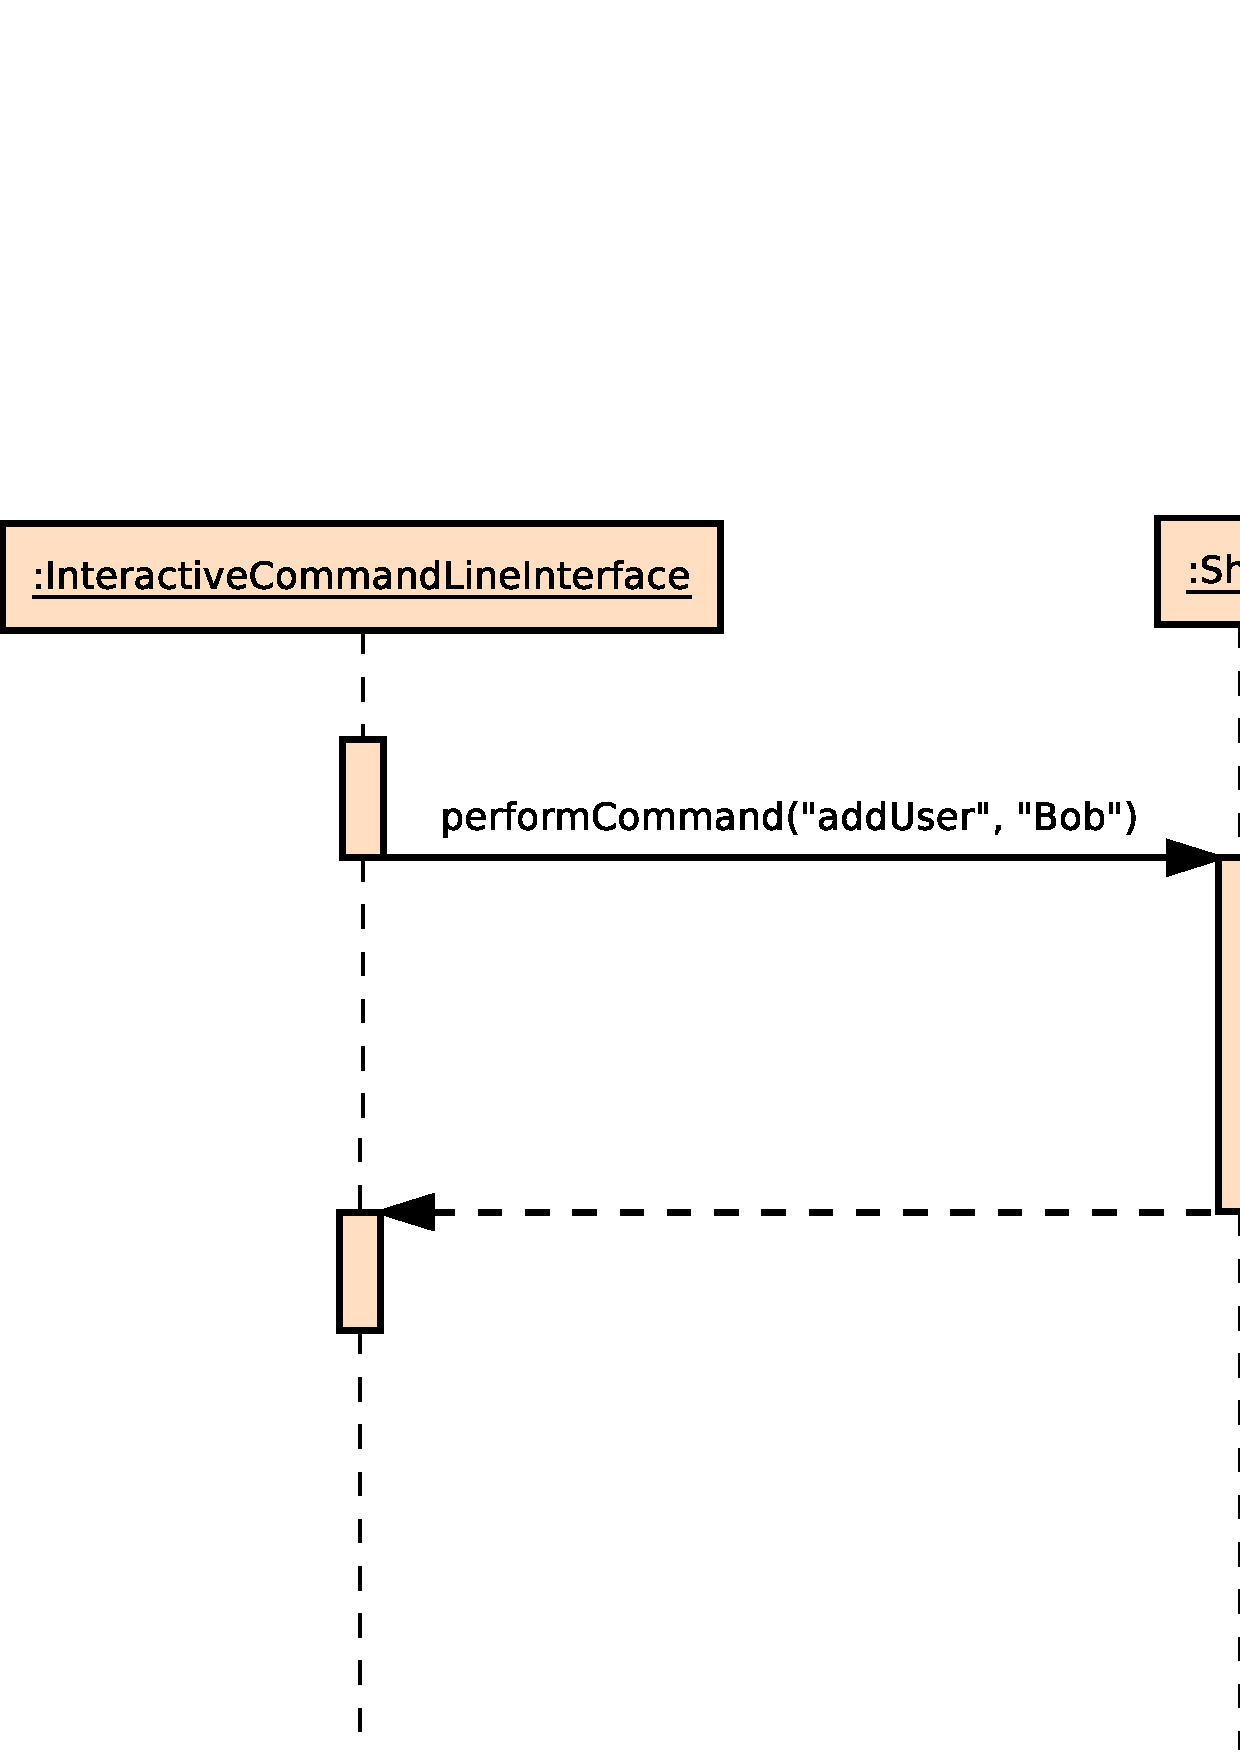
\includegraphics [width=400px] {figures/sequence_diagram_server/Server1.pdf}
\end{illustration}
\begin{illustration}{Sequence diagram of playing a stream for the first time.}
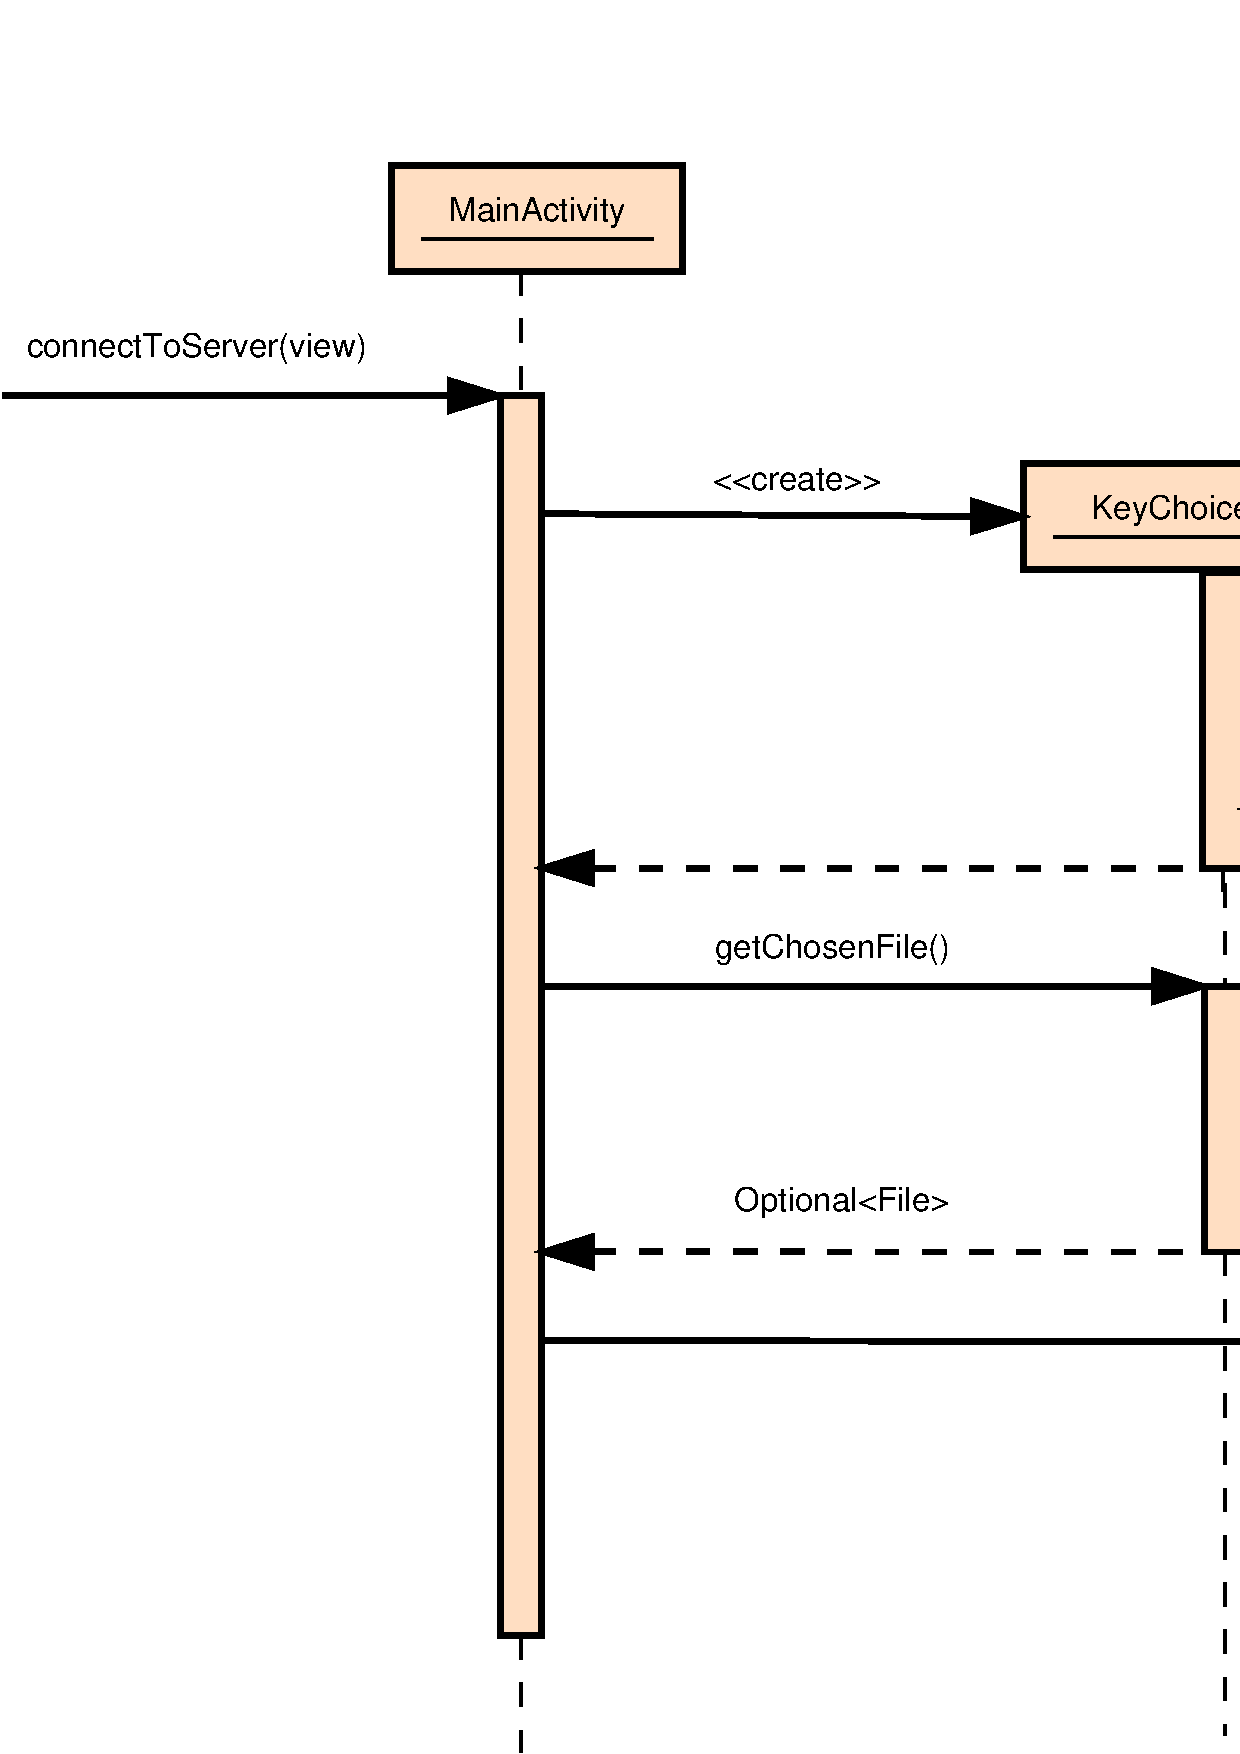
\includegraphics [width=400px] {figures/sequence_diagram_client/sequence_client.pdf}
\end{illustration}

\begin{landscape}
\begin{illustration}{Passing a piece of plaintext data through to the clients (Server side)}
\includegraphics [width=700px] {figures/sequence_diagram_comm1_server/output.pdf}
\end{illustration}
\end{landscape}

\section{GUI design}
The GUI should be user-friendly and intuitional. Therefore its design is very minimalistic, foccusing on its main purpose. 

\subsection{GUI visual examples}
The following images show prototypes of the graphical user interface.

\begin{illustration}{The main screen which is shown on program start.}
\includegraphics[width=150px]{figures/images/mainscreen.png}
\end{illustration}
\begin{illustration}{The menu which pops up after the menu button is pressed. It allows navigation between the different screens.}
\includegraphics[width=150px]{figures/images/menu.png}
\end{illustration}
\begin{illustration}{The option screen which contains preferences, traffic data and a server history.}
\includegraphics[width=150px]{figures/images/optionscreen.png}
\end{illustration}
\begin{illustration}{An example for an error message.}
\includegraphics[width=150px]{figures/images/error.png}
\end{illustration}
\begin{illustration}{The file chooser used for selecting a private key.}
\includegraphics[width=150px]{figures/images/fileChooser.png}
\end{illustration}

\subsection{GUI activity}
\begin{illustration}{Activity diagram showing possible interactions with the program.}
\includegraphics [width=500px]{figures/gui_activity_1/gui_activity_1.png}
\end{illustration}


\section{Time plan}
   \begin{illustration}{A rough time table for the implementation phase}
  \begin{gantt}[xunitlength=0.5cm,fontsize=\small,titlefontsize=\small,drawledgerline=true]{9}{23}
    \begin{ganttitle}
      \titleelement{KW 51}{7}
      \titleelement{KW 2}{7}
      \titleelement{KW 3}{7}
       \titleelement{KW 4}{2}
    \end{ganttitle}
    \begin{ganttitle}
      \numtitle{17}{1}{23}{1}
      \numtitle{7}{1}{22}{1}
    \end{ganttitle}
    \ganttbar[color=yellow]{communication}{0}{3}
    \ganttbar[color=green]{cryptography}{3}{19}
    \ganttbar[color=blue]{server model}{3}{8}
    \ganttbar[color=blue]{server shell}{11}{11}
    \ganttbar[color=red]{client model}{3}{10}
    \ganttbar[color=red]{client view}{13}{9}
    \ganttbar{connect packages}{22}{1}

    \ganttcon{11}{4}{11}{5}
    \ganttcon{13}{6}{13}{7}

    \ganttcon{3}{2}{3}{3}
    \ganttcon{3}{2}{3}{4}
    \ganttcon{3}{2}{3}{6}
    \ganttcon{22}{3}{22}{8}
    \ganttcon{22}{5}{22}{8}
    \ganttcon{22}{7}{22}{8}
  \end{gantt}
  \end{illustration}

\end{document}
